%  --------------------- chapter 4--------------------- %
\chapter{大气运动阻力变化对陆地地表风速长期变化的影响}\label{chap:dragingforceonwind}

\section{引言}

第\ref{chap:drivingforceonwind}章从大气运动驱动力变化的角度分析了陆地地表风速长期变化的原因,本章将从大气运动阻力变化的角度进行分析。

土地利用的变化是大气运动阻力变化的主要原因之一。如第\ref{chap:intro}章所述,已有许多相关研究分析了土地利用变化对于陆地地表风速的影响\citep{vautard2010northern, wu2016estimating, kalnay2003impact, guo2011changes}。以往的研究主要采用对比城市与乡村站点风速变化,建立参考序列与观测序列对比,或是建立简化动力模型和数值模拟的方法。其中,许多以往研究将观测站点分为城市站点和乡村站点(通常是基于人口),通过比较两类站点的风速趋势差别来确定城市化对于风速的影响\citep{guo2011changes}。这种方法能够成立基于以下假设:城市站点周边建设用地增加总是显著快于乡村站点周边,而同时乡村站点周边建设用地增加几乎可以忽略,即人口多的地区的城市化速度显著快于人口少的地区。然而这个假设存在一定问题,更好的方式是通过计算城市人口或建设用地的动态变化来确定城市化的速度。此外,也有研究通过建立不受土地利用变化影响的参考序列,并对比观测序列来考察土地利用变化的影响。有些再分析资料(如NCEP/NCAR)没有同化陆地观测资料,因而被认为可以作为参考序列\citep{kalnay2003impact}。\citet{zha2017effects}将此思路用于了土地利用变化对中国东部地区风速的影响。这种方法能一定程度上反映土地变化的作用,但即便同样是没有同化地表风速观测的再分析资料之间,对于地表风速变化也存在很大分歧(参见第\ref{chap:SpatiotemporalCharacteristics}章),因而这种方法的可靠性也在疑问。另外一种方式是利用简化动力学模型(形式类似于第\ref{chap:intro}章公式 \ref{eq:winddynmaic}),将土地利用的影响简化为拖拽系数的变化(例如\citet{wu2016estimating}),这种简化不一定能够代表土地利用变化对于边界层内湍流混合过程的复杂影响,因而对分析结果造成一定的不确定性。也有研究尝试用数值模拟的手段进行研究,但这些研究多是采用假设的土地利用变化情景而不是真实的土地利用变化进行研究(例如\citet{vautard2010northern})。由此,为了克服前人研究的不足,本章先是利用动态的土地利用数据与风速观测数据进行统计分析,然后设计数值试验考察真实的土地利用变化对于风速的影响。

大气运动的动量由边界层以上的自由大气向边界层内传递主要依赖湍流混合过程。垂直温度递减率是影响湍流强度的主要变量之一,原因是垂直温度递减率的改变会引起大气稳定度变化,当下层增温超过上层时气块会在浮力的作用下形成不稳定运动\citep{J2004An}。\citet{gaffen2000multidecadal}发现,1979-2000年间地表附近的增暖快于对流层低层,表明边界层稳定度增加。据我所知,目前还没有研究分析近几十年来大尺度的边界层垂直温度递减率变化,本章将对这个问题进行分析。

\section{资料和方法}

本章使用了以下数据集:
NCEI-CMDC陆地地表风速观测数据集。此数据集的相关信息已在第二章中做过描述,这里不再重复。本章使用此数据进行大尺度长期风速变化的分析。

中国地面气候资料日值数据集(V3.0)。此数据集同样在第二章中已有介绍。本章将此数据集经过均一化处理后(处理方法将在下文详细介绍)用于珠江三角洲风速长期变化的分析。之所以在此区域的分析中没有使用NCEI-CMDC数据集是由于此数据集由于严格的质量控制过程剔除了大量站点,使得珠江三角洲的风速观测序列只有一个,以此分析珠江三角洲风速长期变化不确定性很大。而相比之下,经过均一化之后的中国地面气候资料日值数据集在珠江三角洲有6个站点,分析结果的不确定性大大降低。

\href{http://www.resdc.cn}{中国土地利用/土地覆盖遥感监测数据集} 由中国科学院资源环境科学数据中心制作,包含20世纪70年代末期、80年代末期、90年代中期、90年代末期、2005年、2010年和2015年7个时期中国土里利用/土地覆盖数据,空间分辨率为1 $\times$ 1 km。此数据集使用Landsat遥感影像数据制作而成,包含耕地、林地、草地、水域、城乡工矿居民用地、未利用土地6个大类和25各小类。本章使用了20世纪70年代末和2015年土地利用数据作为数值模拟的边界条件进行珠江三角洲城市化对于风速长期变化影响的数值试验。

MODIS12Q1土地利用数据集\citep{sullamenashe2019hierarchical}由美国宇航局(NASA)制作,包含全球2001年至今每年500 $\times$ 500 m分辨率土地利用数据。此数据集使用Terra和Aqua卫星上搭载的中分辨率成像光谱仪(MODIS)传感器数据制作而成,包含IGBP、UMD、LAI、BGC和PFT5个分类标准下的土地利用数据。本章使用了2001年和2016年土地利用数据作为数值模拟的边界条件进行芬兰南部植被变化对于风速长期变化影响的数值试验。

\href{http://www.atlasofurbanexpansion.org/data}{Atlas of Urban Expansion城市变化数据集} 由纽约大学(NYU)制作,包含20世纪80年代至21世纪前10年全球200个城市发展的动态数据,包括人口、城市建设面积、街区和道路等。此数据集使用Landsat遥感影像数据制作而成。本章使用了全球200个城市的城市建设面积动态数据分析城市化与风速长期变化的关系。

\href{https://climatedataguide.ucar.edu/climate-data/ndvi-normalized-difference-vegetation-index-3rd-generation-nasagfsc-gimms}{GIMMS NDVI 3g}由NASA制作,包含全球1981年至2015年0.083 $\times$ 0.083度归一化植被指数(NDVI)数据。此数据集由卫星上搭载的超高分辨率辐射计(AVHRR)数据制作而成,NDVI计算公式如下:

\begin{equation} \label{eq:ndvi}
NDVI = \frac{NIR - VIS}{NIR + VIS}
\end{equation} ~\\
其中NIR表示近红外光反射率,VIS表示可见光反射率。健康的植被会吸收大部分可见光,而反射大部分近红外光,然而不健康或者稀疏的植被会反射更多可见光和更少近红外光。NDVI的范围是-1 \textasciitilde 1,当没有绿叶存在时NDVI接近与0,当绿叶密度非常高时NDVI接近1。本章使用1982和2015年NDVI数据分析植被变化与风速长期变化的关系。

HadGHCND全球地表温度观测数据集\citep{caesar2006large-scale}由哈德莱中心制作,包含全球1950年至今2.5纬度$\times$3.75经度分辨率日最高和最低温度观测数据。此数据集由NCEI等全球历史气候网络(GHCN)日观测数据集制作而成,制作过程中包含了质量控制步骤以减少错误和可疑数据等影响,并使用角度-距离加权算法将站点数据差值到格点。本章使用1979-2012年地表日最高气温分析边界层日间垂直温度递减率变化。

HadAT全球对流层温度数据集\citep{thorne2005revisiting}由哈德莱中心制作,包含全球1985-2012年5纬度$\times$10经度分辨率对流层850、700、500、300、200、150、100、50和30 hPa共9个层次的月平均温度。此数据集由676个探空站点数据制作而成,由于这些探空站点多分布于北半球,因而此数据集有效数据也多集中于北半球。制作过程中使用了质量控制步骤来减小仪器和观测方式等变化的影响。本章使用了1979-2012年850 hPa温度数据分析边界层垂直温度递减率的变化。

本章使用了RHtest V4观测序列均一化算法\citep{wang2014rhtests}对风速观测序列进行均一化处理。此算法基于penalized maximal t test\citep{wang2007penalized}和penalized maximal F test\citep{wang2008penalized},可以在有参考序列和没有参考序列的情况下检测观测序列的异常突变点,并进行修正,修正方式包括均值修正和Quantile-Matching(QM)修正,后者既可以调整均值也可以使突变点前后的经验分布一致\citep{wang2010new},获得广泛应用\citep{vincent2012second, baule2014climatology, yang2019causes}。本章在处理珠江三角洲风速数据时使用ERA-Interim 10 m风场资料作为参考序列检测观测序列的突变点,并使用QM修正,最后用人工检查确认突变点检测和修正无明显不当之处。

本章数值试验使用了WRF-ARW 4.0\citep{skamarock2019description},此模式是由美国国家大气研究中心(NCAR)开发的下一代中尺度数值天气预测系统,是目前模拟效果最好、应用最广泛的中尺度天气数值模式。本章的数值试验使用FNL作为初始和边界条件,分别针对城市化和植被变化在珠江三角洲和芬兰南部进行了两组数值试验,模式参数设置和数值试验设计将在下文中详细描述。

本章计算趋势和相关系数以及统计显著性水平的方法与第\ref{chap:SpatiotemporalCharacteristics}、\ref{chap:drivingforceonwind}章相同。RMSD计算方法如下:

\begin{equation} \label{eq:rmsd}
RMSD = \frac{\frac{1}{N} \sum_{n=1}^{N} \left( c_{n} - \bar{c} \right) \left( d_{n} - \bar{d} \right) }{\sigma_{c} \sigma_{d}}
\end{equation} ~\\
其中$\bar{c}$和$\bar{d}$分别为空间场c和d的均值,$\sigma_{c}$和$\sigma_{d}$为c和d的标准差。

\section{城市化的影响} \label{sec:urbanimpact}

\subsection{基于城市动态变化和风速观测数据的统计学分析}

\begin{figure}[!htbp]
    \centering
    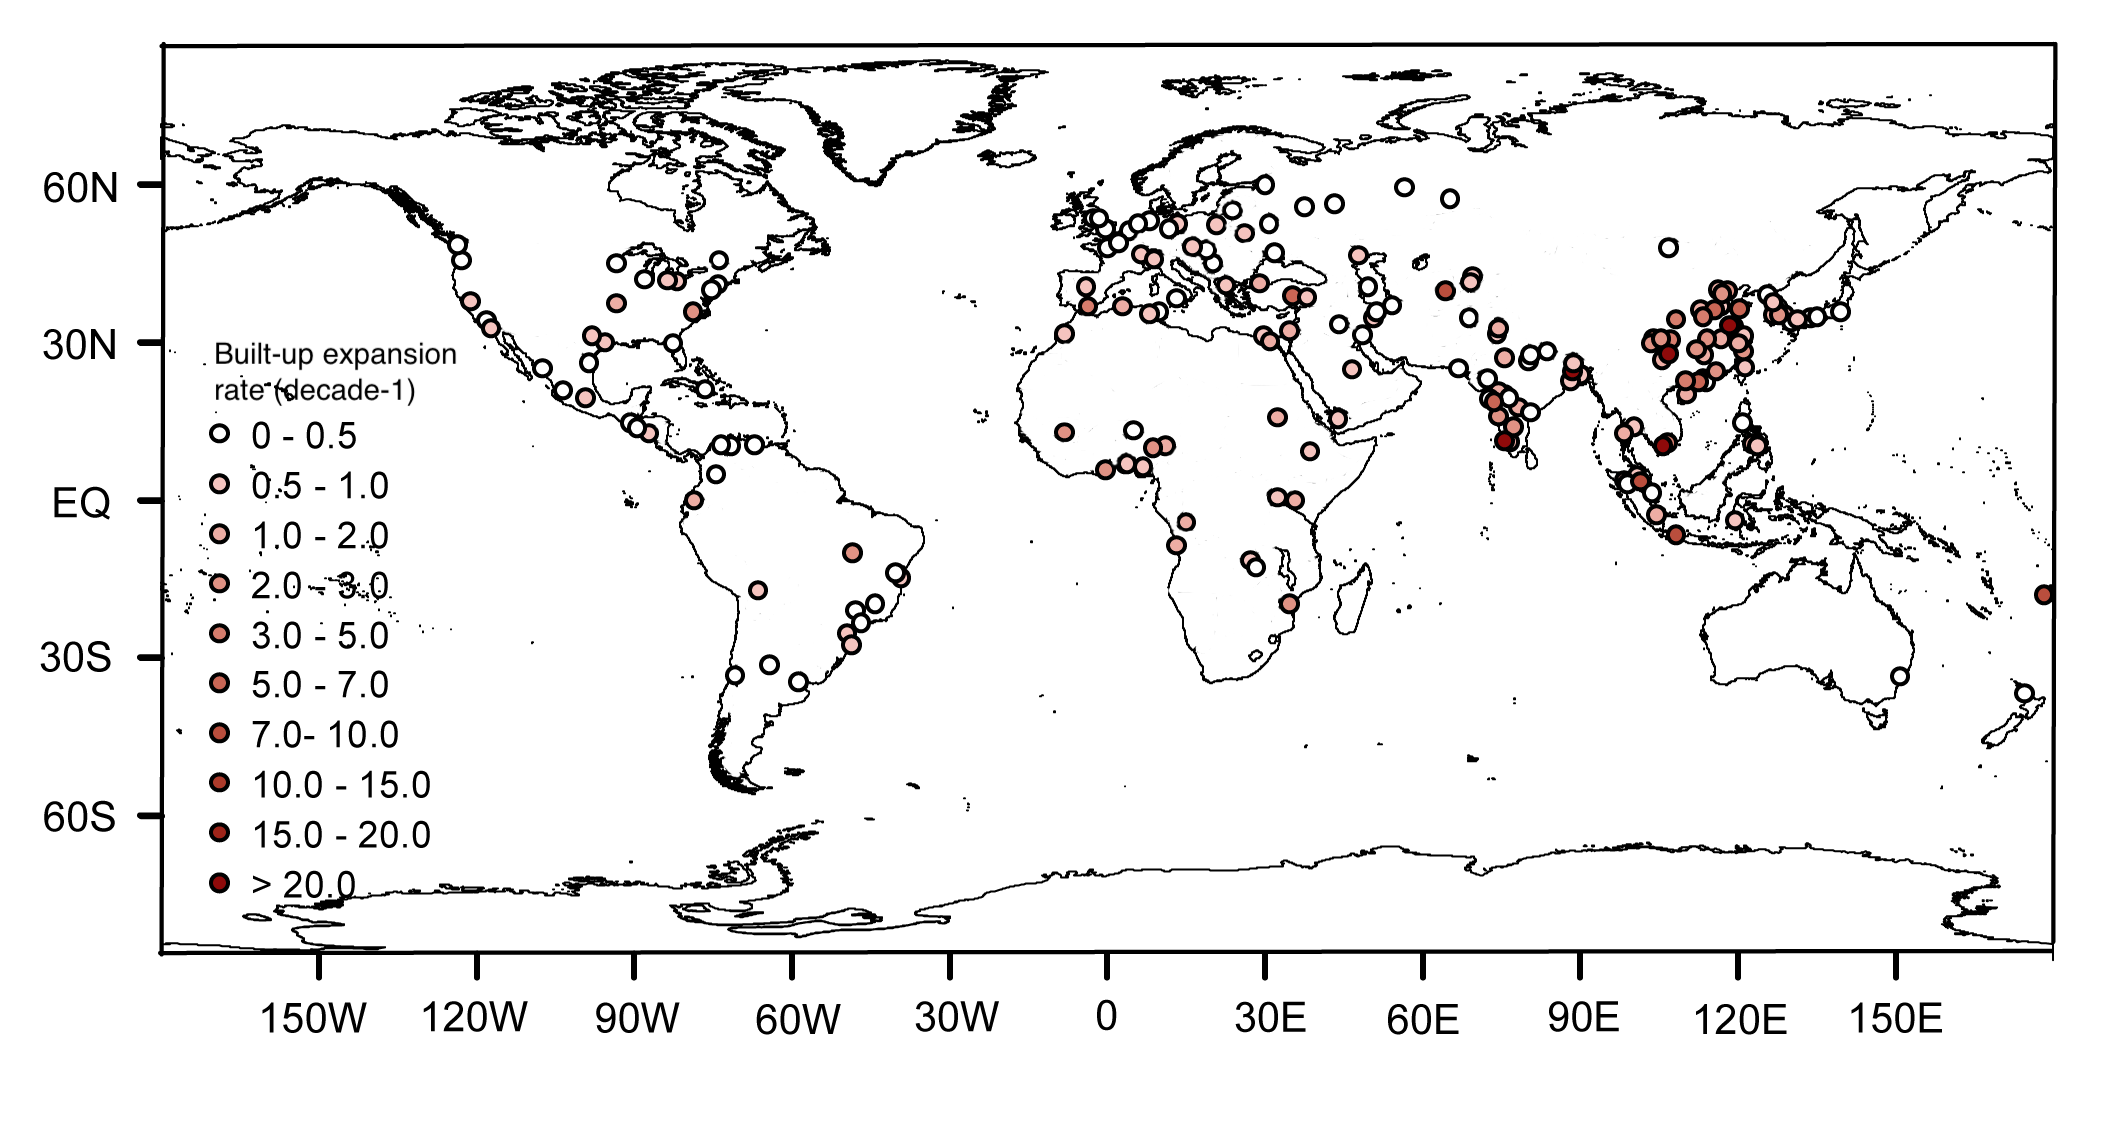
\includegraphics[width=1\textwidth]{城市扩张速度}
    \bicaption{ 城市扩张速度(变化率 每十年)}{City expansion rate (in $changing ~ rate ~ per ~ decade$)}
    \label{fig:cityexpansionrate}
\end{figure}

%\setupctable{captionsleft}% 标题朝向
\begin{figure}[!htbp]
    \centering
    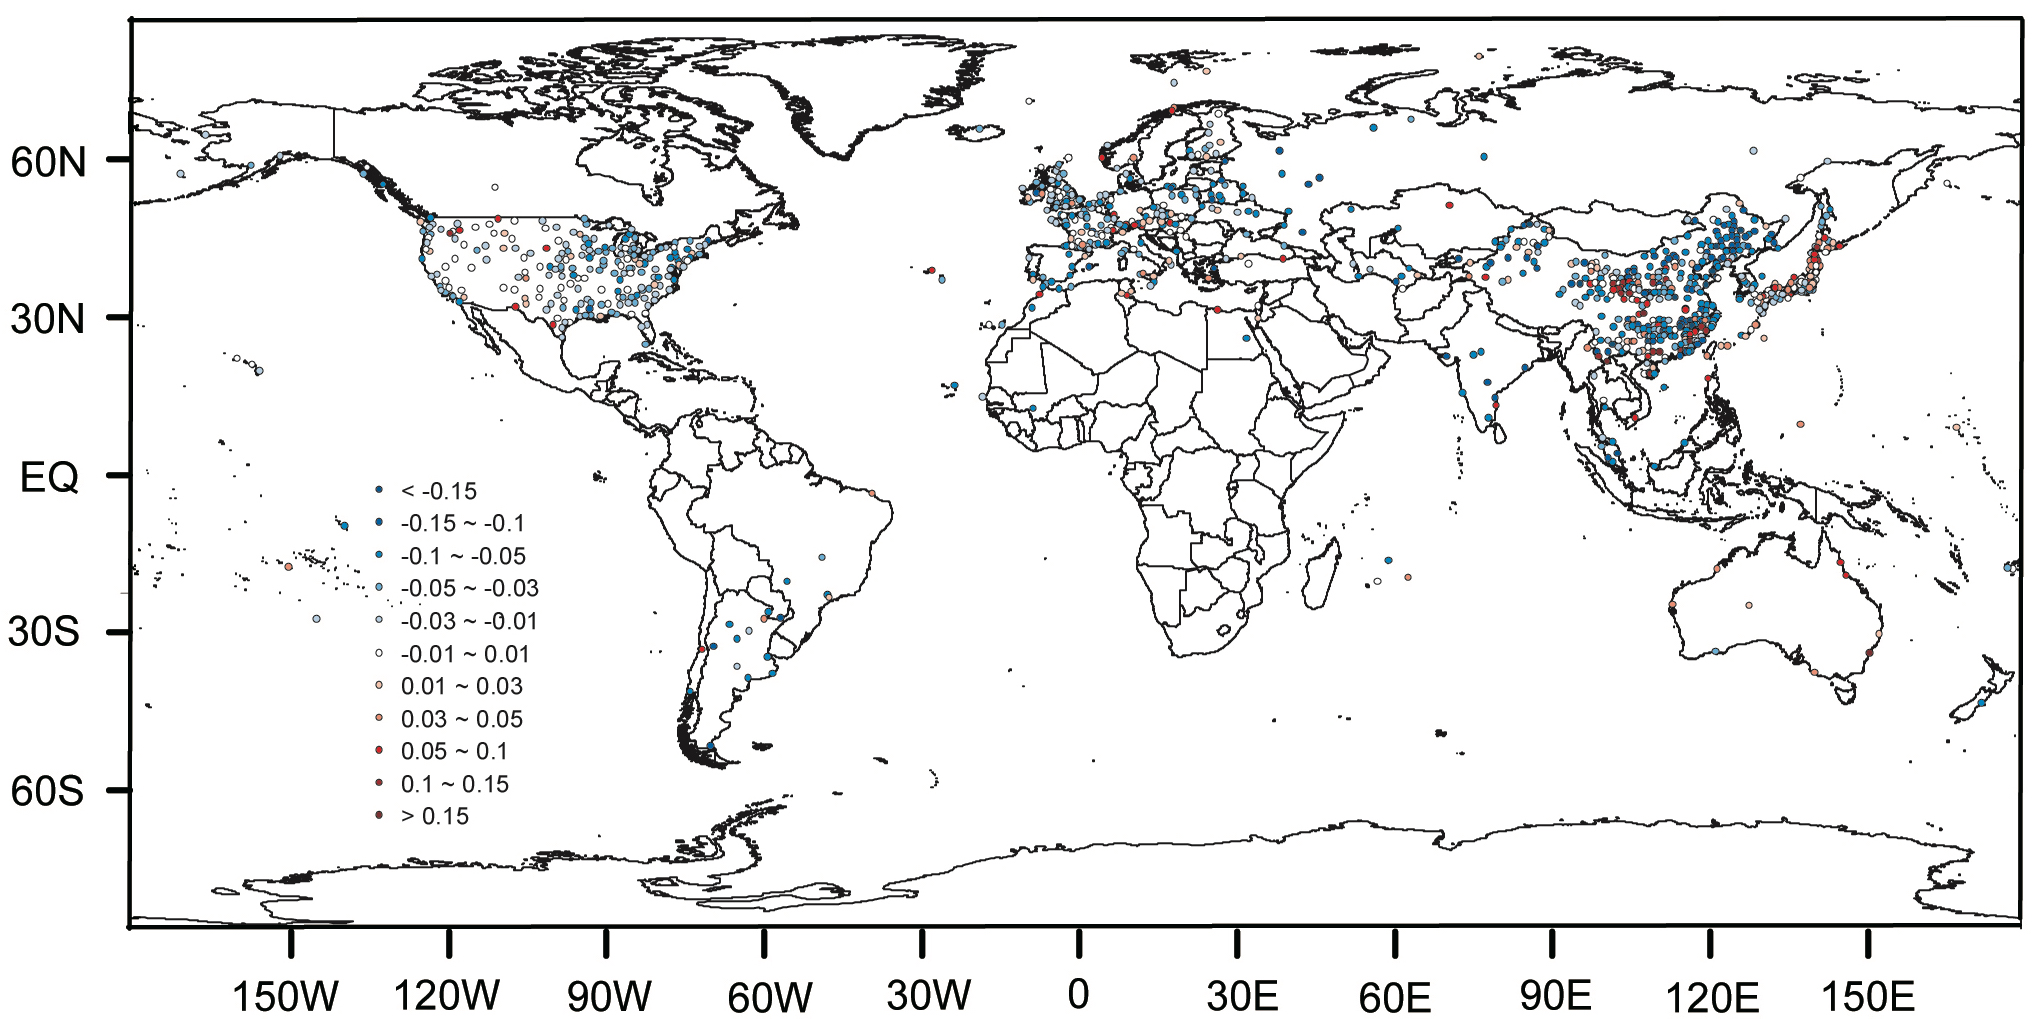
\includegraphics[width=1\textwidth]{归一化地表风速趋势}
    \bicaption{ 归一化地表风速趋势(变化率 每十年)}{Normalized surface wind speed trends (in $changing ~ rate ~ per ~ decade$)}
     \label{fig:normalizedwindtrend}
\end{figure}

\begin{figure}[!htbp]
    \centering
    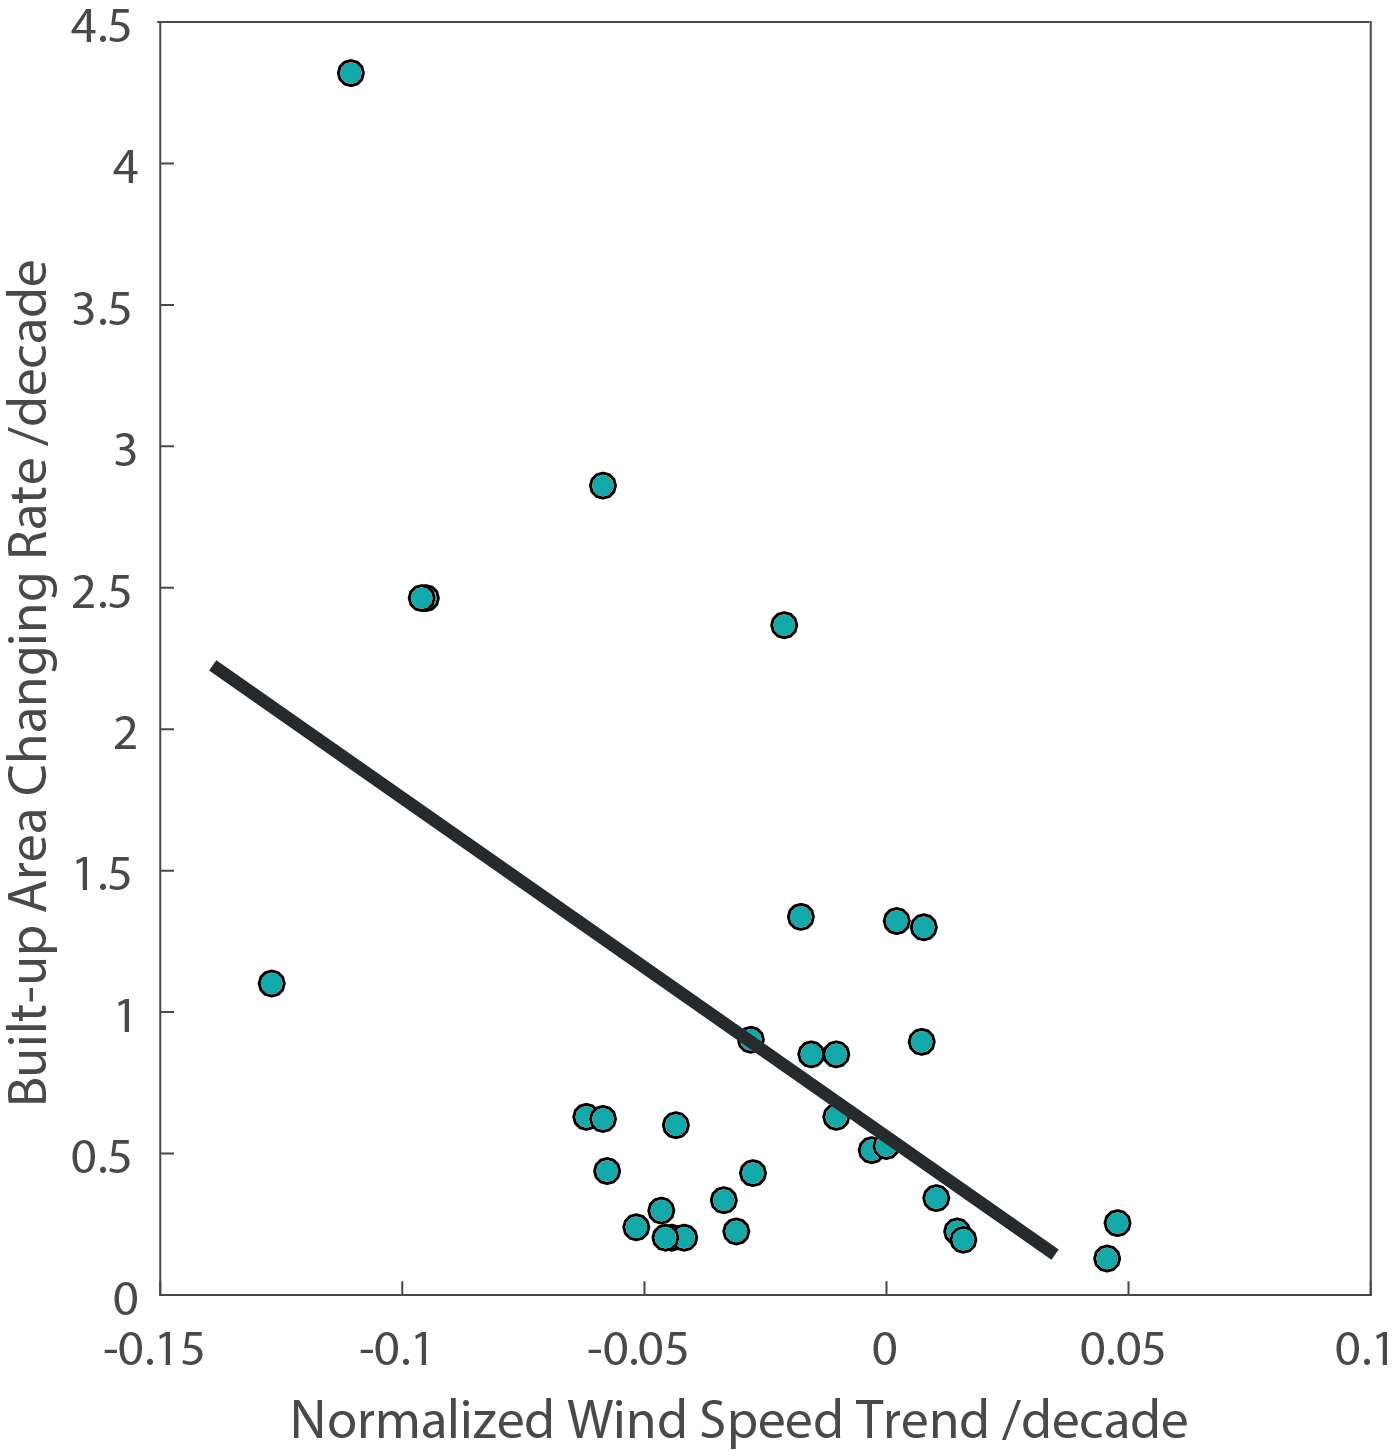
\includegraphics[width=0.5\textwidth]{城市扩张与风速变化}
    \bicaption{ 城市扩张速度与对应地区风速变化}{City expansion versus wind speed change in the corresponding area.}
    \label{fig:cityexpansionvswindchange}
\end{figure}

\begin{figure}[!htbp]
    \centering
    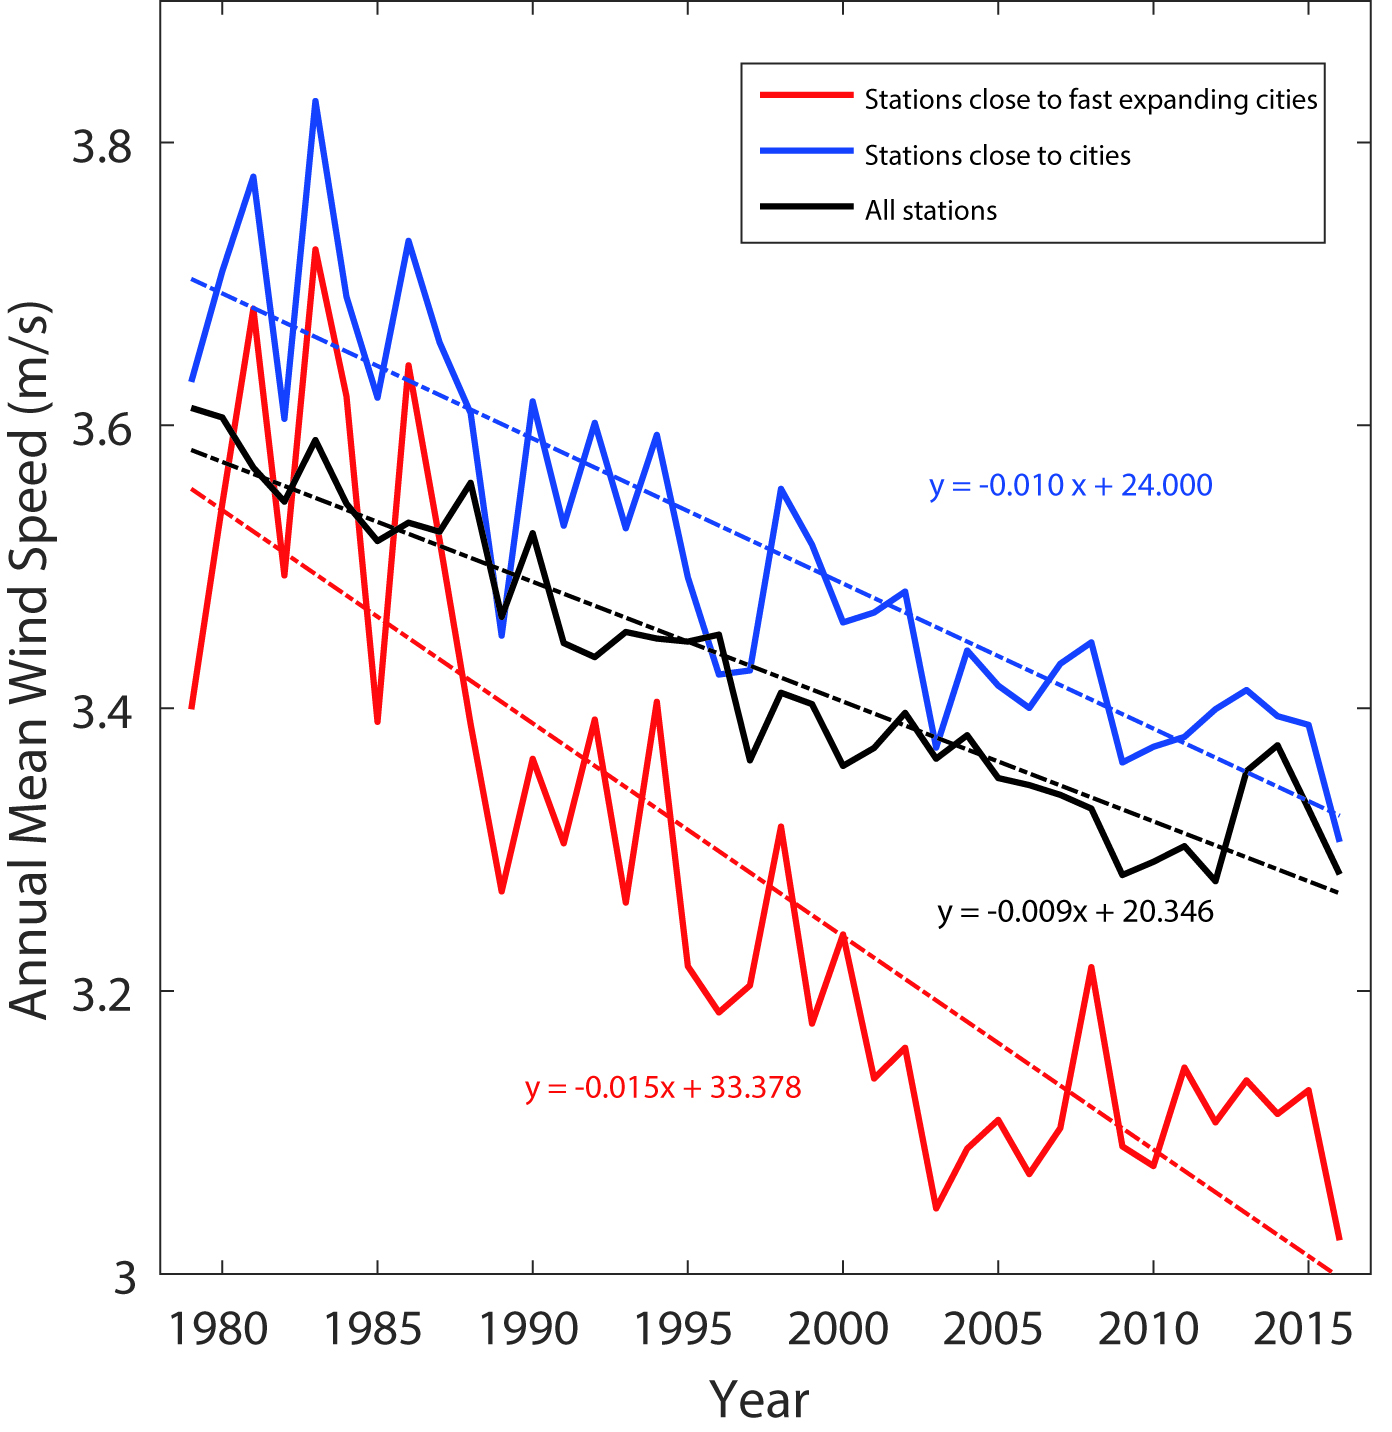
\includegraphics[width=0.5\textwidth]{不同城市化速度风速对比}
    \bicaption{ 不同城市化速度地区风速演变。红色实线为快速城市化的城市附近站点风速演变,蓝色实线为所有靠近城市站点风速演变,黑色实线为所有站点风速演变。虚线为对应实线的线性趋势。}{Wind speed evolution under different urbanization rates. Red solid line is evolution of wind speed near fast urbanizing cities, blue solid line is evolution of wind speed near all cities, black solid line is evolution of wind speed across the world. Dash lines are trends for solid lines.}
    \label{fig:windunderdiffurban}
\end{figure}

使用Atlas of Urban Expansion数据计算城市建设面积自20世纪80年代至21世纪前10年的变化率,发现所有200个城市建设面积都有增加,其中62\%增加速度超过50\% 每十年,36\%超过100\% 每十年,增加最快的中国江苏盱城和孟加拉国Rajshahi增加速度超过4000\% 每十年。相比之下,北美洲和欧洲城市建设面积增加速度较慢,原因是欧美发达国家的城市化在更早时候就已经基本完成,而亚洲的中国、印度和东南亚各国,近30多年来城市化进程非常迅速(图 \ref{fig:cityexpansionrate})。对比使用NCEI-CMDC风速数据计算的1979-2016年归一化风速趋势,发现亚洲整体风速下降速度大于欧洲和北美(图 \ref{fig:normalizedwindtrend}),似乎预示着城市化在其中起到了一定作用。选择距离城市中心0.15度(约15 km)以内的观测站点,将地表风速趋势与城市建设面积变化速度对比,发现二者有显著的负相关(p < 0.01),即城市扩张越快的地区,风速越趋向于减小(图 \ref{fig:cityexpansionvswindchange})。对比上述城市中心附近站点中城市扩张速度在前50\%的风速趋势,所有城市中心附近站点风速趋势和所有站点风速趋势发现,所有城市中心附近站点和所有站点平均风速趋势接近,分别为0.1 和 0.09 $m ~ s^{-1}$每十年,相比之下快速扩张城市周边站点平均风速趋势则得多,达到0.15 $m ~ s^{-1}$每十年(图 \ref{fig:windunderdiffurban})。由此说明城市化进程会使得附近的风速显著减小。

\subsection{数值试验}

为了进一步验证城市化与风速变化的关系,使用WRF-ARW 4.0进行数值试验,选择中国东南沿海的珠江入海口附近的珠江三角洲作为模拟区域(图 \ref{fig:PRDlocation}),因为它包含广州、深圳、珠海、香港、澳门等城市,是中国中国近30多年来城市化最快的地区之一(图 \ref{fig:PRDcityexpand}),而中国是全球近30多年来城市化最快的国家之一。此地区地势较为平坦,海拔高度基本在800 m以下 (图 \ref{fig:PRDlocation})。

\begin{figure}[!htbp]
    \centering
    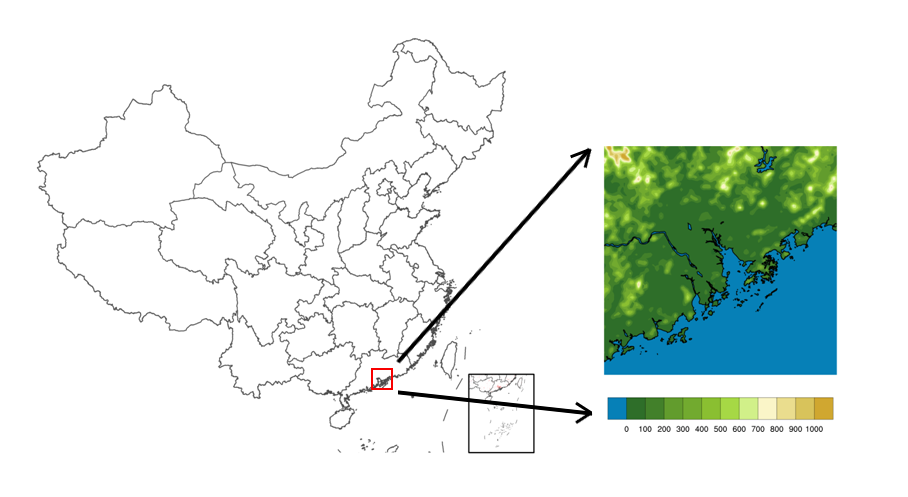
\includegraphics[width=1\textwidth]{珠江三角洲地理位置}
    \bicaption{ 珠江三角洲地理位置}{Location of the Pearl River Delta.}
    \label{fig:PRDlocation}
\end{figure}

\begin{figure}[!t]
    \centering
    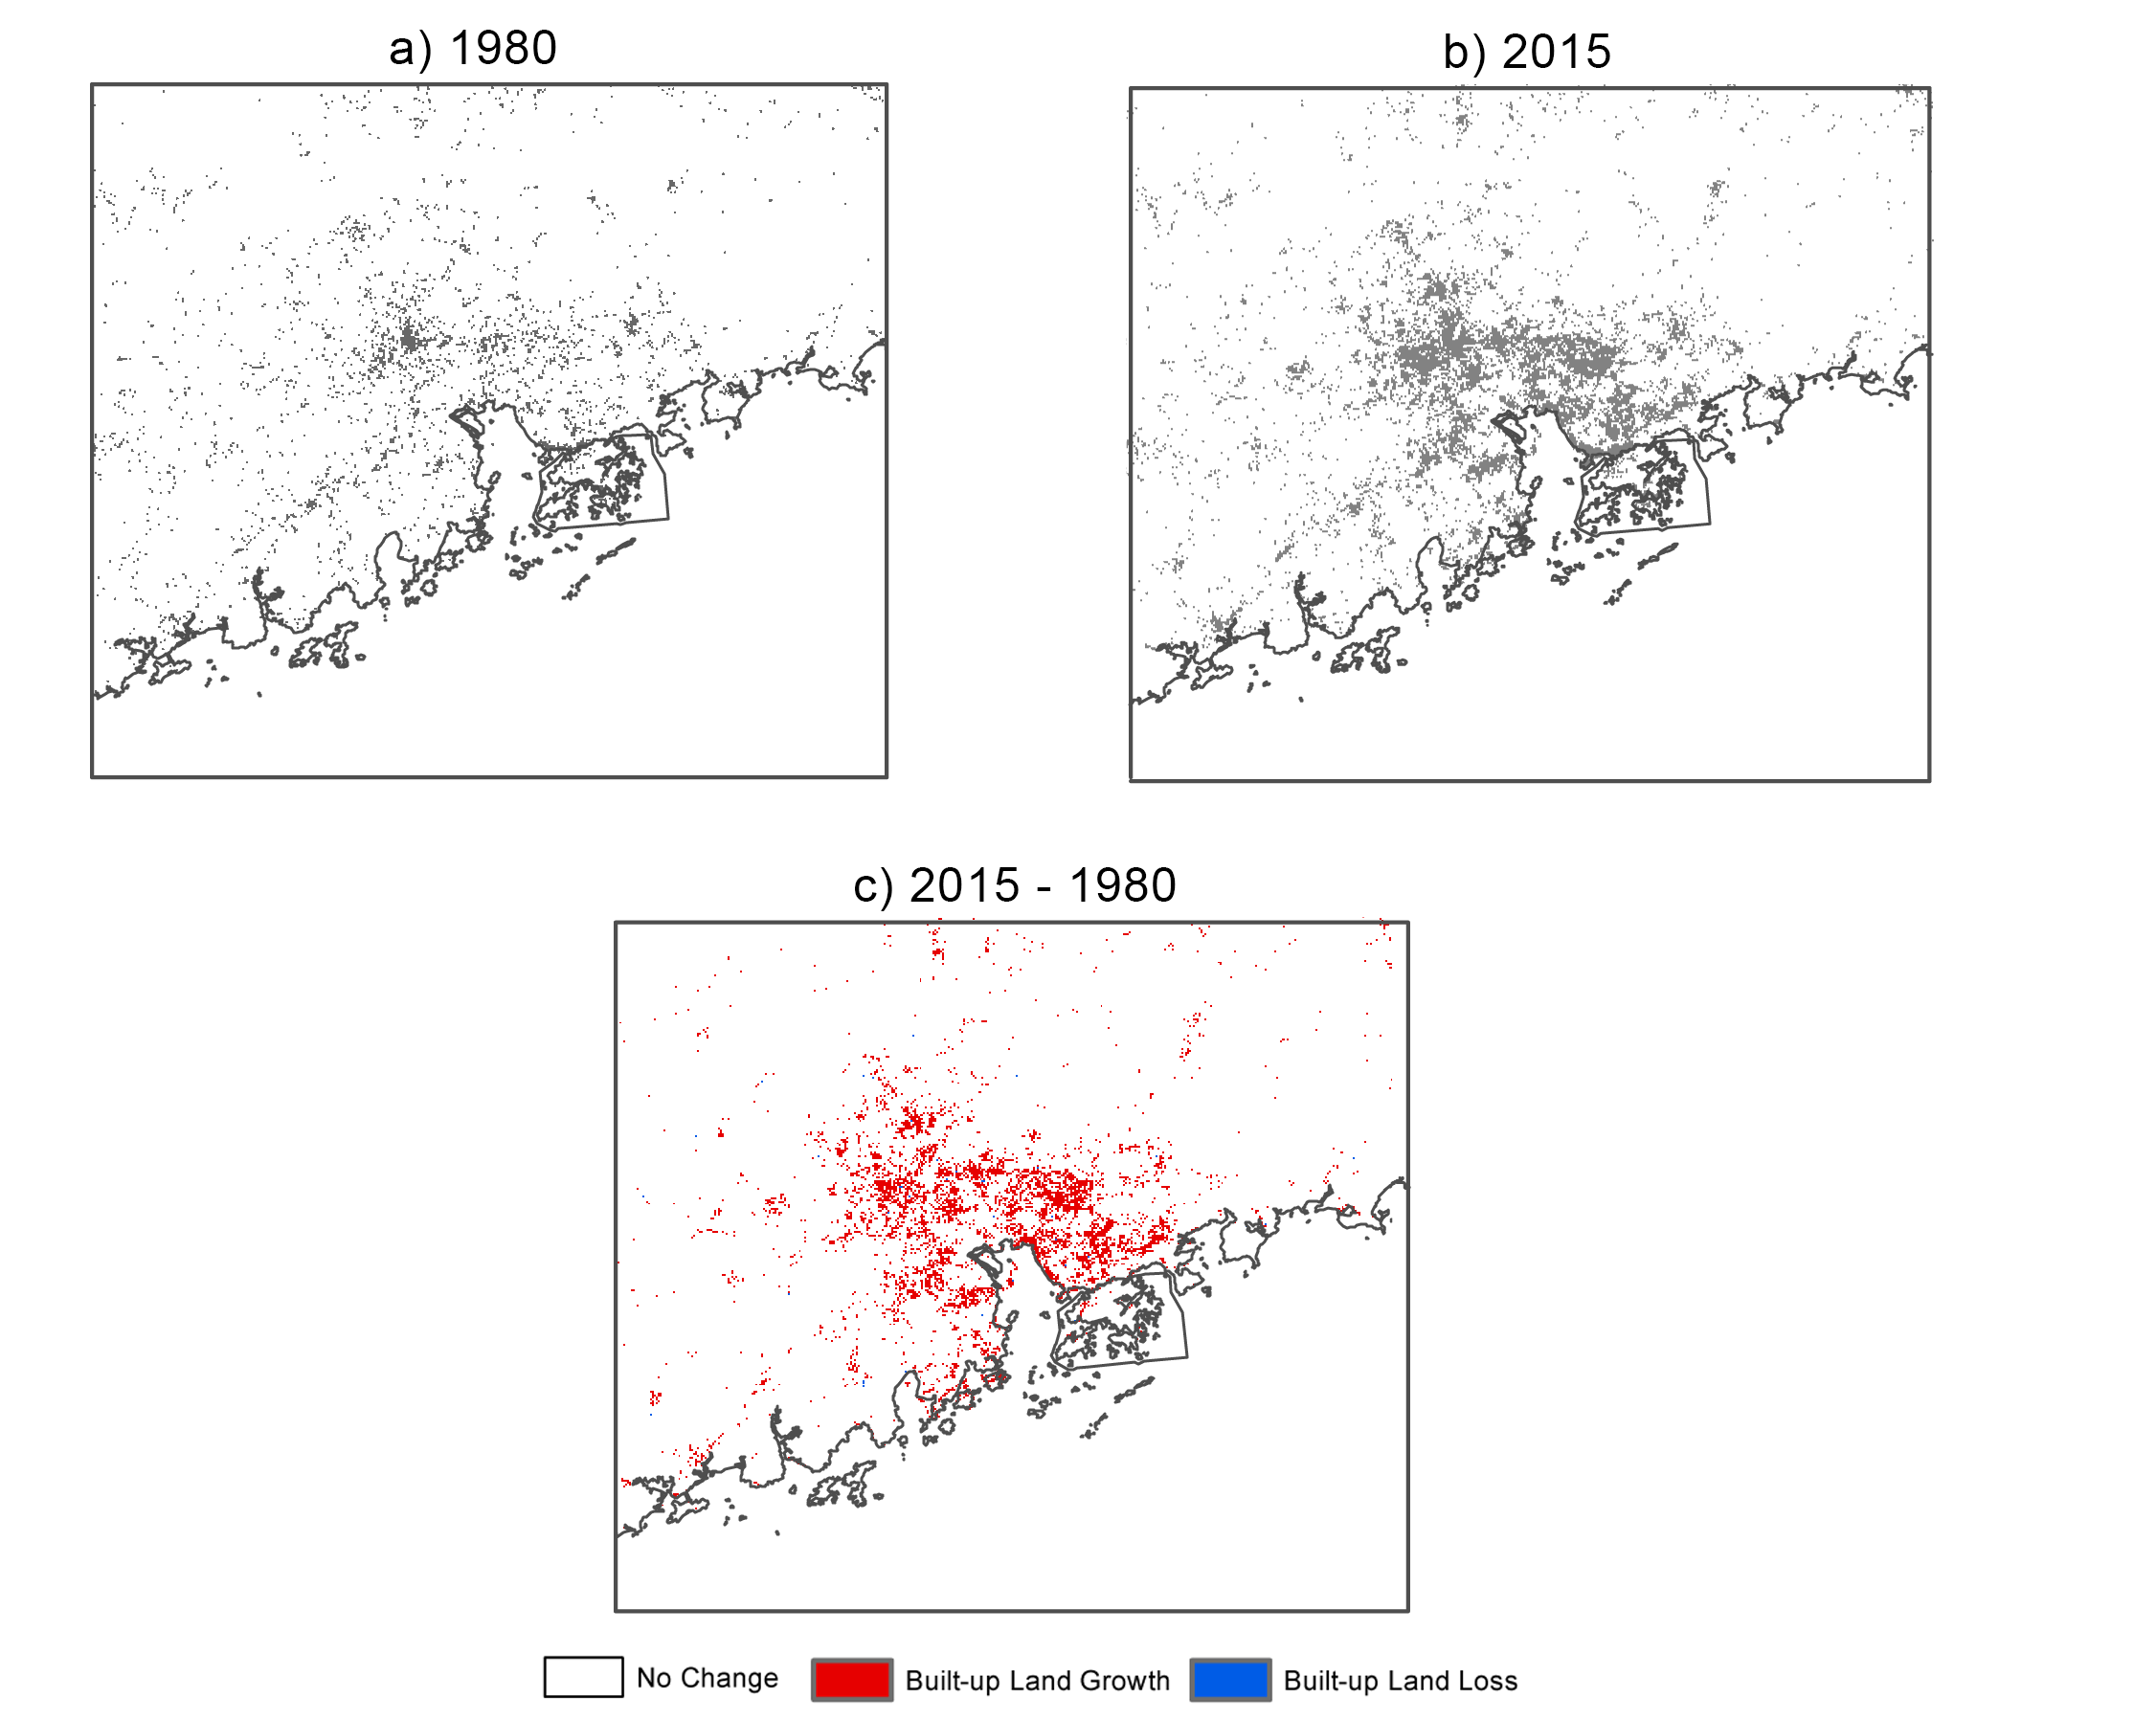
\includegraphics[width=1\textwidth]{珠江三角洲城市扩张}
    \bicaption{ 珠江三角洲城市扩张。a)1980年城市范围,b)2015年城市范围,c)2015年相对1980年城市范围的变化,白色表示没有变化,红色表示增加,蓝色表示减少。}{City expansion in the Pearl River Delta. a)Built-up extension in 1980, b)Built-up extension in 2015, c)Built-up change from 1980 to 2015, white color denotes no change occurred, red denotes add, blue denotes lose.}
    \label{fig:PRDcityexpand}
\end{figure}

将模式设置为三层双向嵌套,空间分辨率分别为30km、10km和3.3km(图 \ref{fig:PRDmodeldomain}),垂直包含40个层次,其中边界层内(1km高度以下)10个层次;时间步长为100 s;微物理参数化方案为WRF Single-Moment 6-class scheme;积云参数化方案为Grell 3D,在较高分辨率的两层网格关闭积云参数化;云量使用Xu-Randall method;长波辐射参数化方案为RRTM scheme,短波辐射参数化方案为Dudhia scheme;边界层采用BouLac PBL,地面层采用Eta similarity,陆面模式选择Noah-MP;城市参数化方案采用Building Environment Parameterization (BEP)。

\begin{figure}[!htbp]
    \centering
    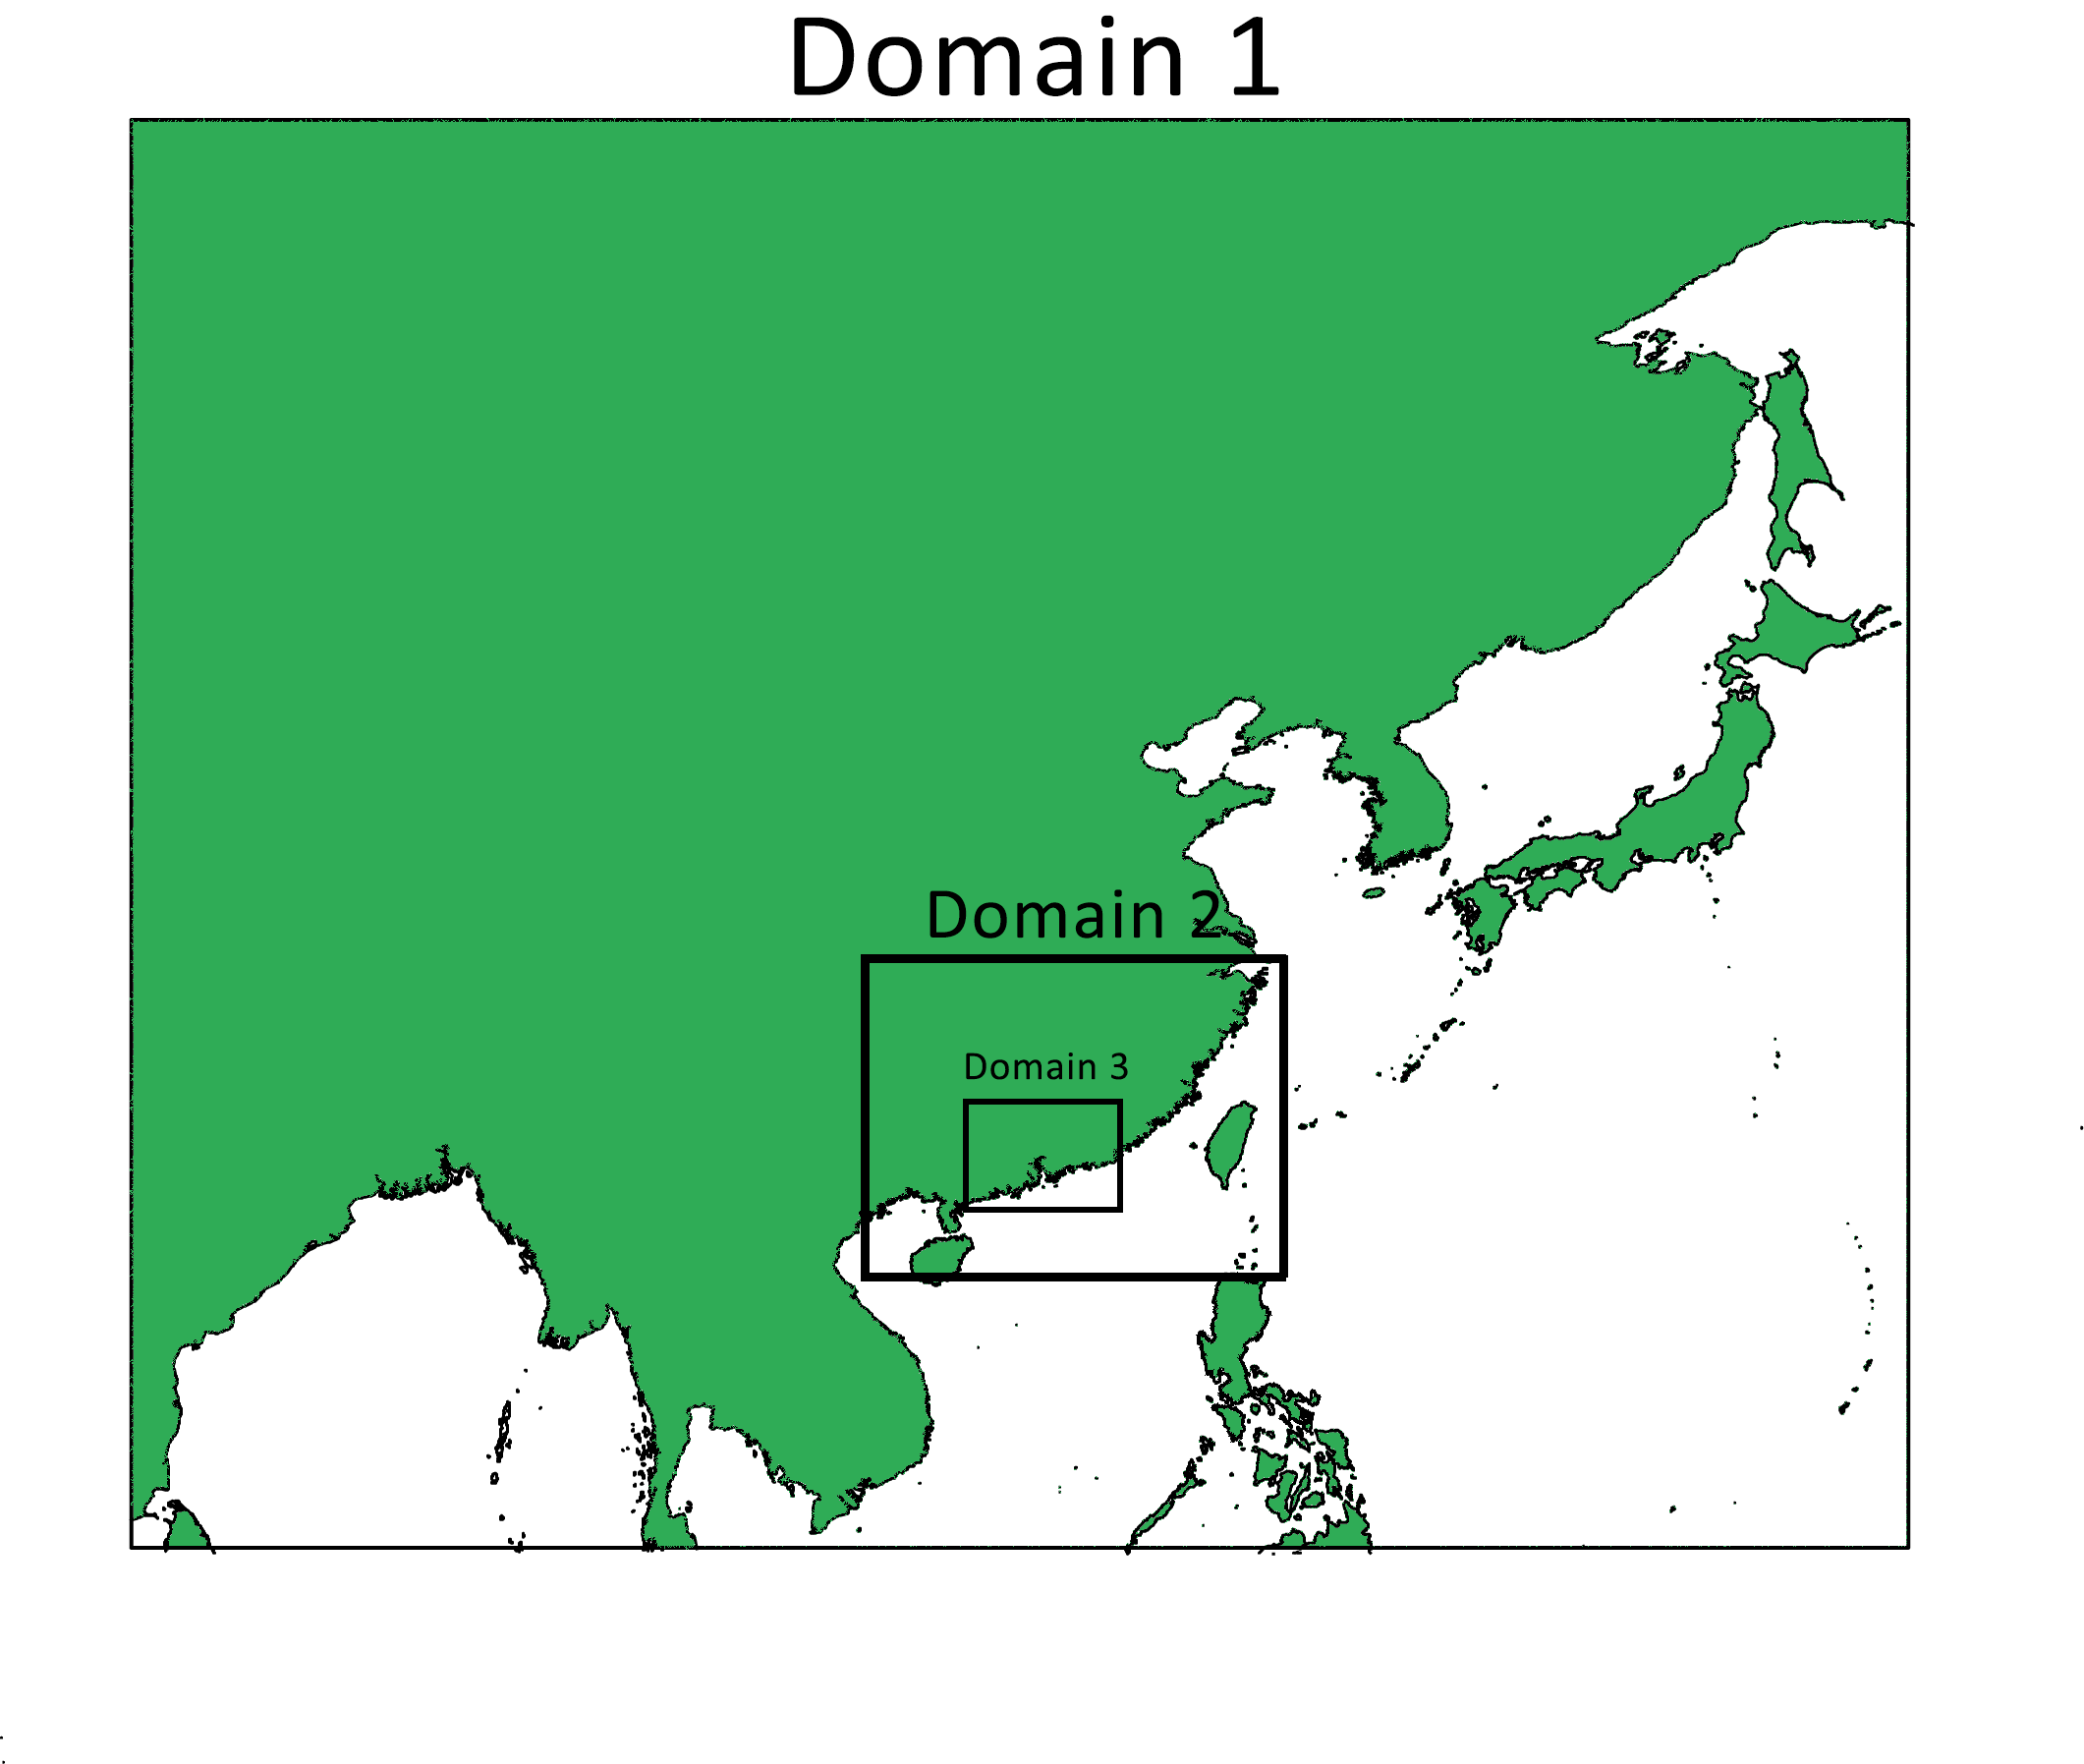
\includegraphics[width=0.7\textwidth]{模拟区域}
    \bicaption{模拟区域}{Model simulation domains}
    \label{fig:PRDmodeldomain}
\end{figure}

采用以上模式设置进行三组模拟,分别为:

\begin{enumerate}

\item \label{sim:1.1} 以华南地区20世纪70年代末土地利用类型(来自中国土地利用/土地覆盖遥感监测数据集)作为下边界条件进行模拟。

\item \label{sim:1.2} 以华南地区20世纪70年代末土地利用类型叠加2015年珠江三角洲地区建设用地范围作为下边界条件进行模拟。
	
\item \label{sim:1.3} 以华南地区2015年土地利用类型作为下边界条件进行模拟。

\end{enumerate}

对以上三组模拟,气象场采用FNL2015年6月和2015年12月(分别代表珠江三角洲雨季和旱季)1 $\times$ 1度6小时分辨率物理量场,经确认,在模拟时段内无台风和寒潮过程发生。

\begin{figure}[!htbp]
    \centering
    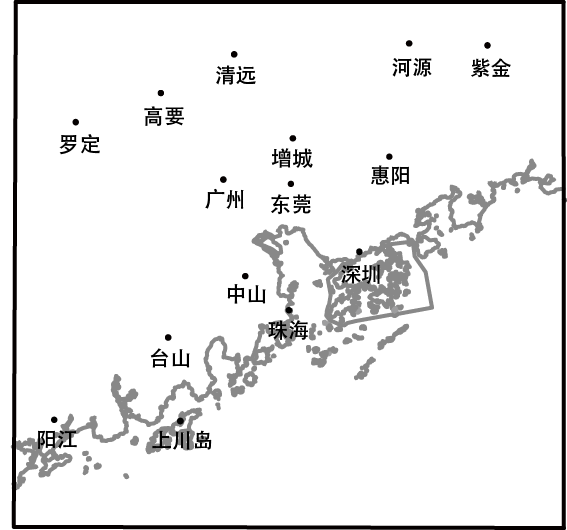
\includegraphics[width=0.5\textwidth]{珠江三角洲测站位置}
    \bicaption{ 珠江三角洲测站位置}{Observation stations in the Pearl River Delta.}
    \label{fig:PRDobssites}
\end{figure}

使用模拟\ref{sim:1.3}结果对比观测进行模式性能评估,珠江三角洲及周边区域地面观测站点位置和信息可在图 \ref{fig:PRDobssites}和表 \ref{tab:PRDsiteinfo}找到。对比模拟与观测结果,发现模拟风速普遍大于观测,这在以往的研究中也被发现\citep{zhang2010modeling, yu2015evaluation, zha2019numerical}。为了减少这种模拟偏差的影响,在模拟结果的分析时,应使用归一化风速变化而不是风速变化的绝对值。模拟与观测风速体现出了很好的相关,说明模拟结果可以很大程度上抓住风速的时间变化。RMSD结果对比以往研究\citep{zhang2010modeling, zha2019numerical}也表明模式对珠江三角洲区域风速有较好的模拟效果(表 \ref{tab:PRDsiteinfo})。

\begin{table}[!htbp]
    \bicaption{珠江三角洲站点信息及模式性能评估结果}{Description of observation stations in the Pearl River Delta and model validation results}
    \label{tab:PRDsiteinfo}
    \centering
    \small% fontsize
    \setlength{\tabcolsep}{5 pt}% column separation
    \renewcommand{\arraystretch}{1.0}%row space 
    \begin{tabular}{lccccccc}
        \hline
        站名 & 站号 & 纬度 & 经度 & 海拔(m)&  \multicolumn{3}{c}{10 m 风速} \\
         & & & & & 均值($m ~ s^{-1}$)$^*$ &  相关系数 $^ {**}$ & RMSD \\
        %\cline{2-9}% partial hline from column i to column j
        \hline
        高要 & 59278 & 23.02 & 112.27 & 41.9 & 3.7(-1.8) & 0.07 & 1.21 \\
        清远 & 59280 & 23.43 & 113.05 & 79.2 & 3.4(0.1) & \textbf{0.39} & 0.95 \\
        广州 & 59287 & 23.13 & 113.29 & 70.7 & 2.9(-0.4) & \textbf{0.40} & 0.65 \\
        东莞 & 59289 & 22.58 & 113.44 & 56.8 & 2.3(0.5) & \textbf{0.44} & 0.54 \\
        河源 & 59293 & 23.48 & 114.44 & 71.6 & 4.1(-2.1) & \textbf{0.59} & 1.10 \\
        增城 & 59294 & 23.20 & 113.50 & 31.5 & 4.4(-2.0) & \textbf{0.34} & 1.40 \\
        惠阳 & 59298 & 23.04 & 114.22 & 109.3 & 3.2(-0.6) & \textbf{0.55} & 1.23 \\
	   紫金 & 59304 & 23.38 & 115.11 & 177.6 & 3.0(-1.4) & \textbf{0.38} & 0.77 \\
	   罗定 & 59462 & 22.42 & 111.36 & 60.9 & 2.3(-0.7) & 0.21 & 0.89 \\
	   台山 & 59478 & 22.15 & 112.47 & 33.7 & 4.0(-1.4) & \textbf{0.47} & 0.70 \\
	   中山 & 59485 & 22.3 & 113.24 & 34.5 & 3.2(-1.0) & \textbf{0.35} & 0.87 \\
	   珠海 & 59488 & 22.17 & 113.34 & 52.3 & 6.7(-4.2) & \textbf{0.41} & 1.69\\
	   深圳 & 59493 & 22.32 & 114.00 & 63.9 & 3.6(-1.2) & \textbf{0.45} & 1.42 \\
	   阳江 & 59663 & 21.5 & 111.58 & 90.8 & 4.2(-0.1) & 0.30 & 0.90 \\
	   上川岛 & 59673 & 21.44 & 112.46 & 22.3 & 5.5(0.0) & \textbf{0.48} & 1.66 \\    
        \hline
    \end{tabular}
     \vspace*{3ex}
    \begin{minipage}{0.9\textwidth}% choose width suitably
    注:$^*$ 括号外数值为模拟结果,括号内为观测减去模拟。\\ 
    $^{**}$ 加粗的数值代表 p < 0.01。r = 0.33 对应 p = 0.01, r = 0.25 对应 p = 0.05。
    \end{minipage}
\end{table}

\begin{figure}[!t]
    \centering
    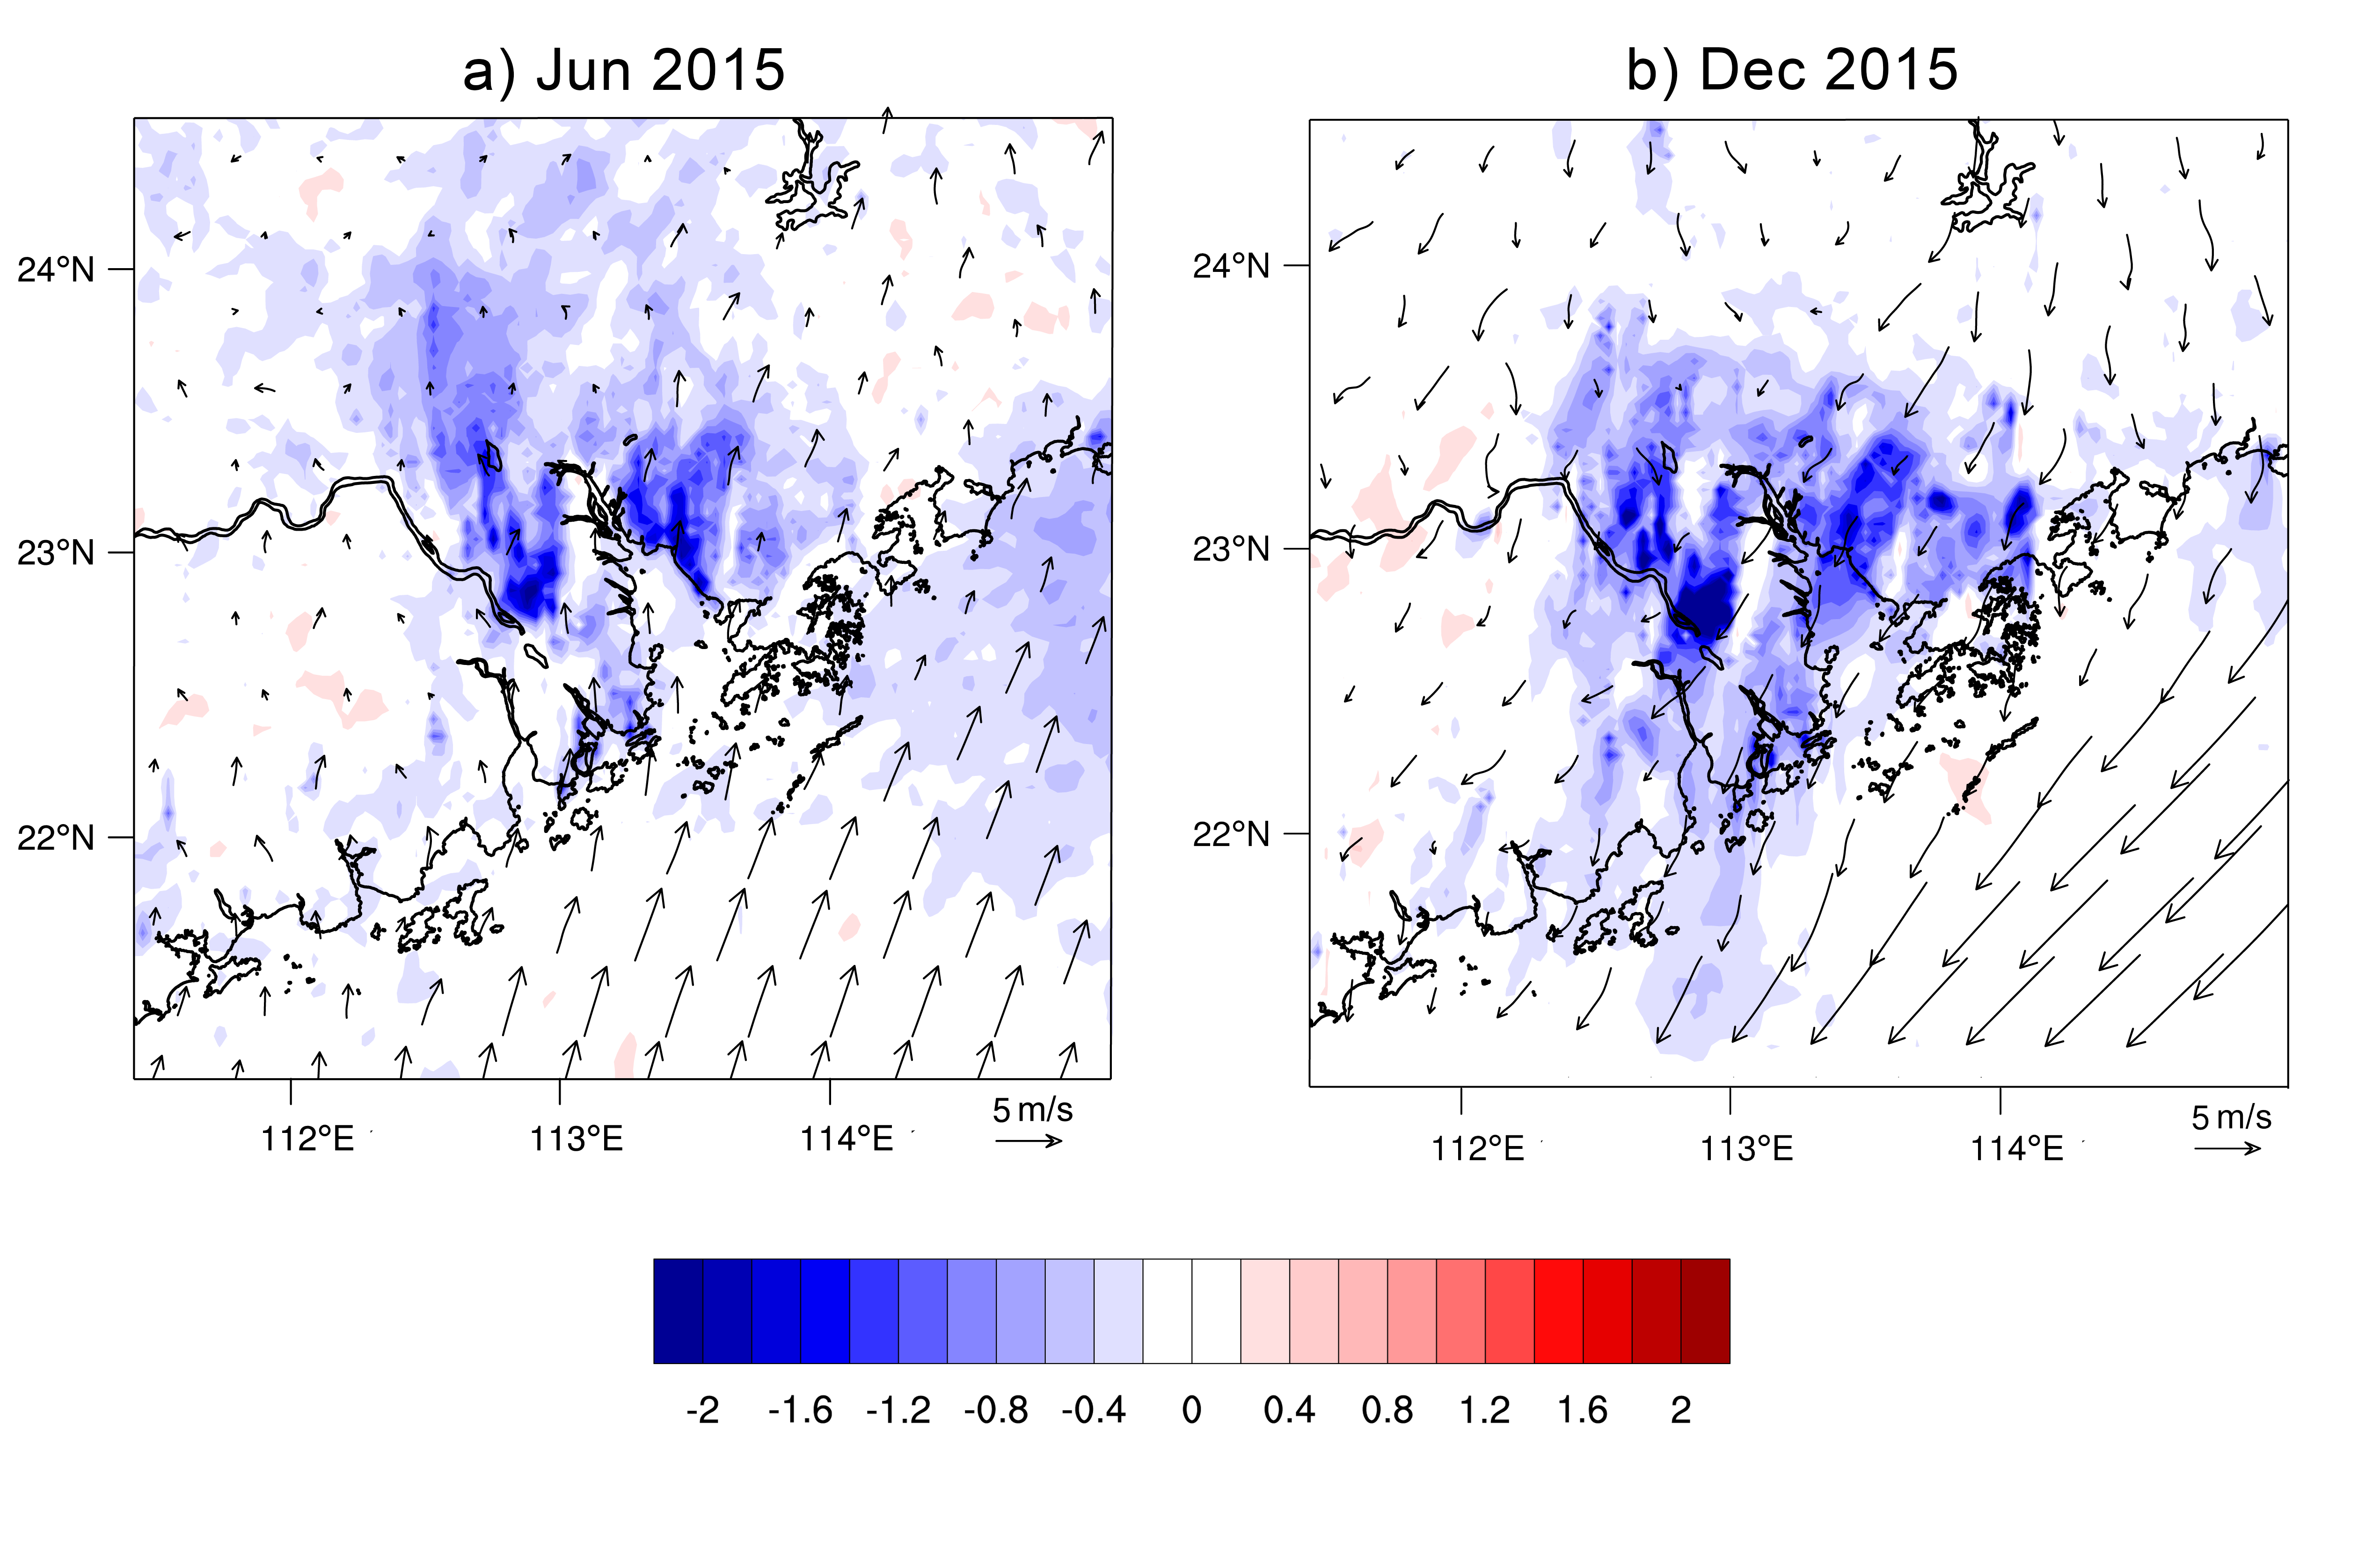
\includegraphics[width=0.9\textwidth]{城市化对地表风速的影响}
    \bicaption{ 城市化对地表风速的影响($m ~ s^{-1}$)。a)使用2015年6月气象场模拟结果,b)使用2015年12月气象场模拟结果,矢量箭头为对应时间背景风矢量。}{Impact of urbanization on surface wind speed (in $m ~ s^{-1}$). a)Model simulation using June 2015 meteorological fields, b)Model simulation using December 2015 meteorological fields, vectors are background wind vectors during corresponding periods.}
    \label{fig:urbanizationonwind}
\end{figure}

\begin{figure}[!b]
    \centering
    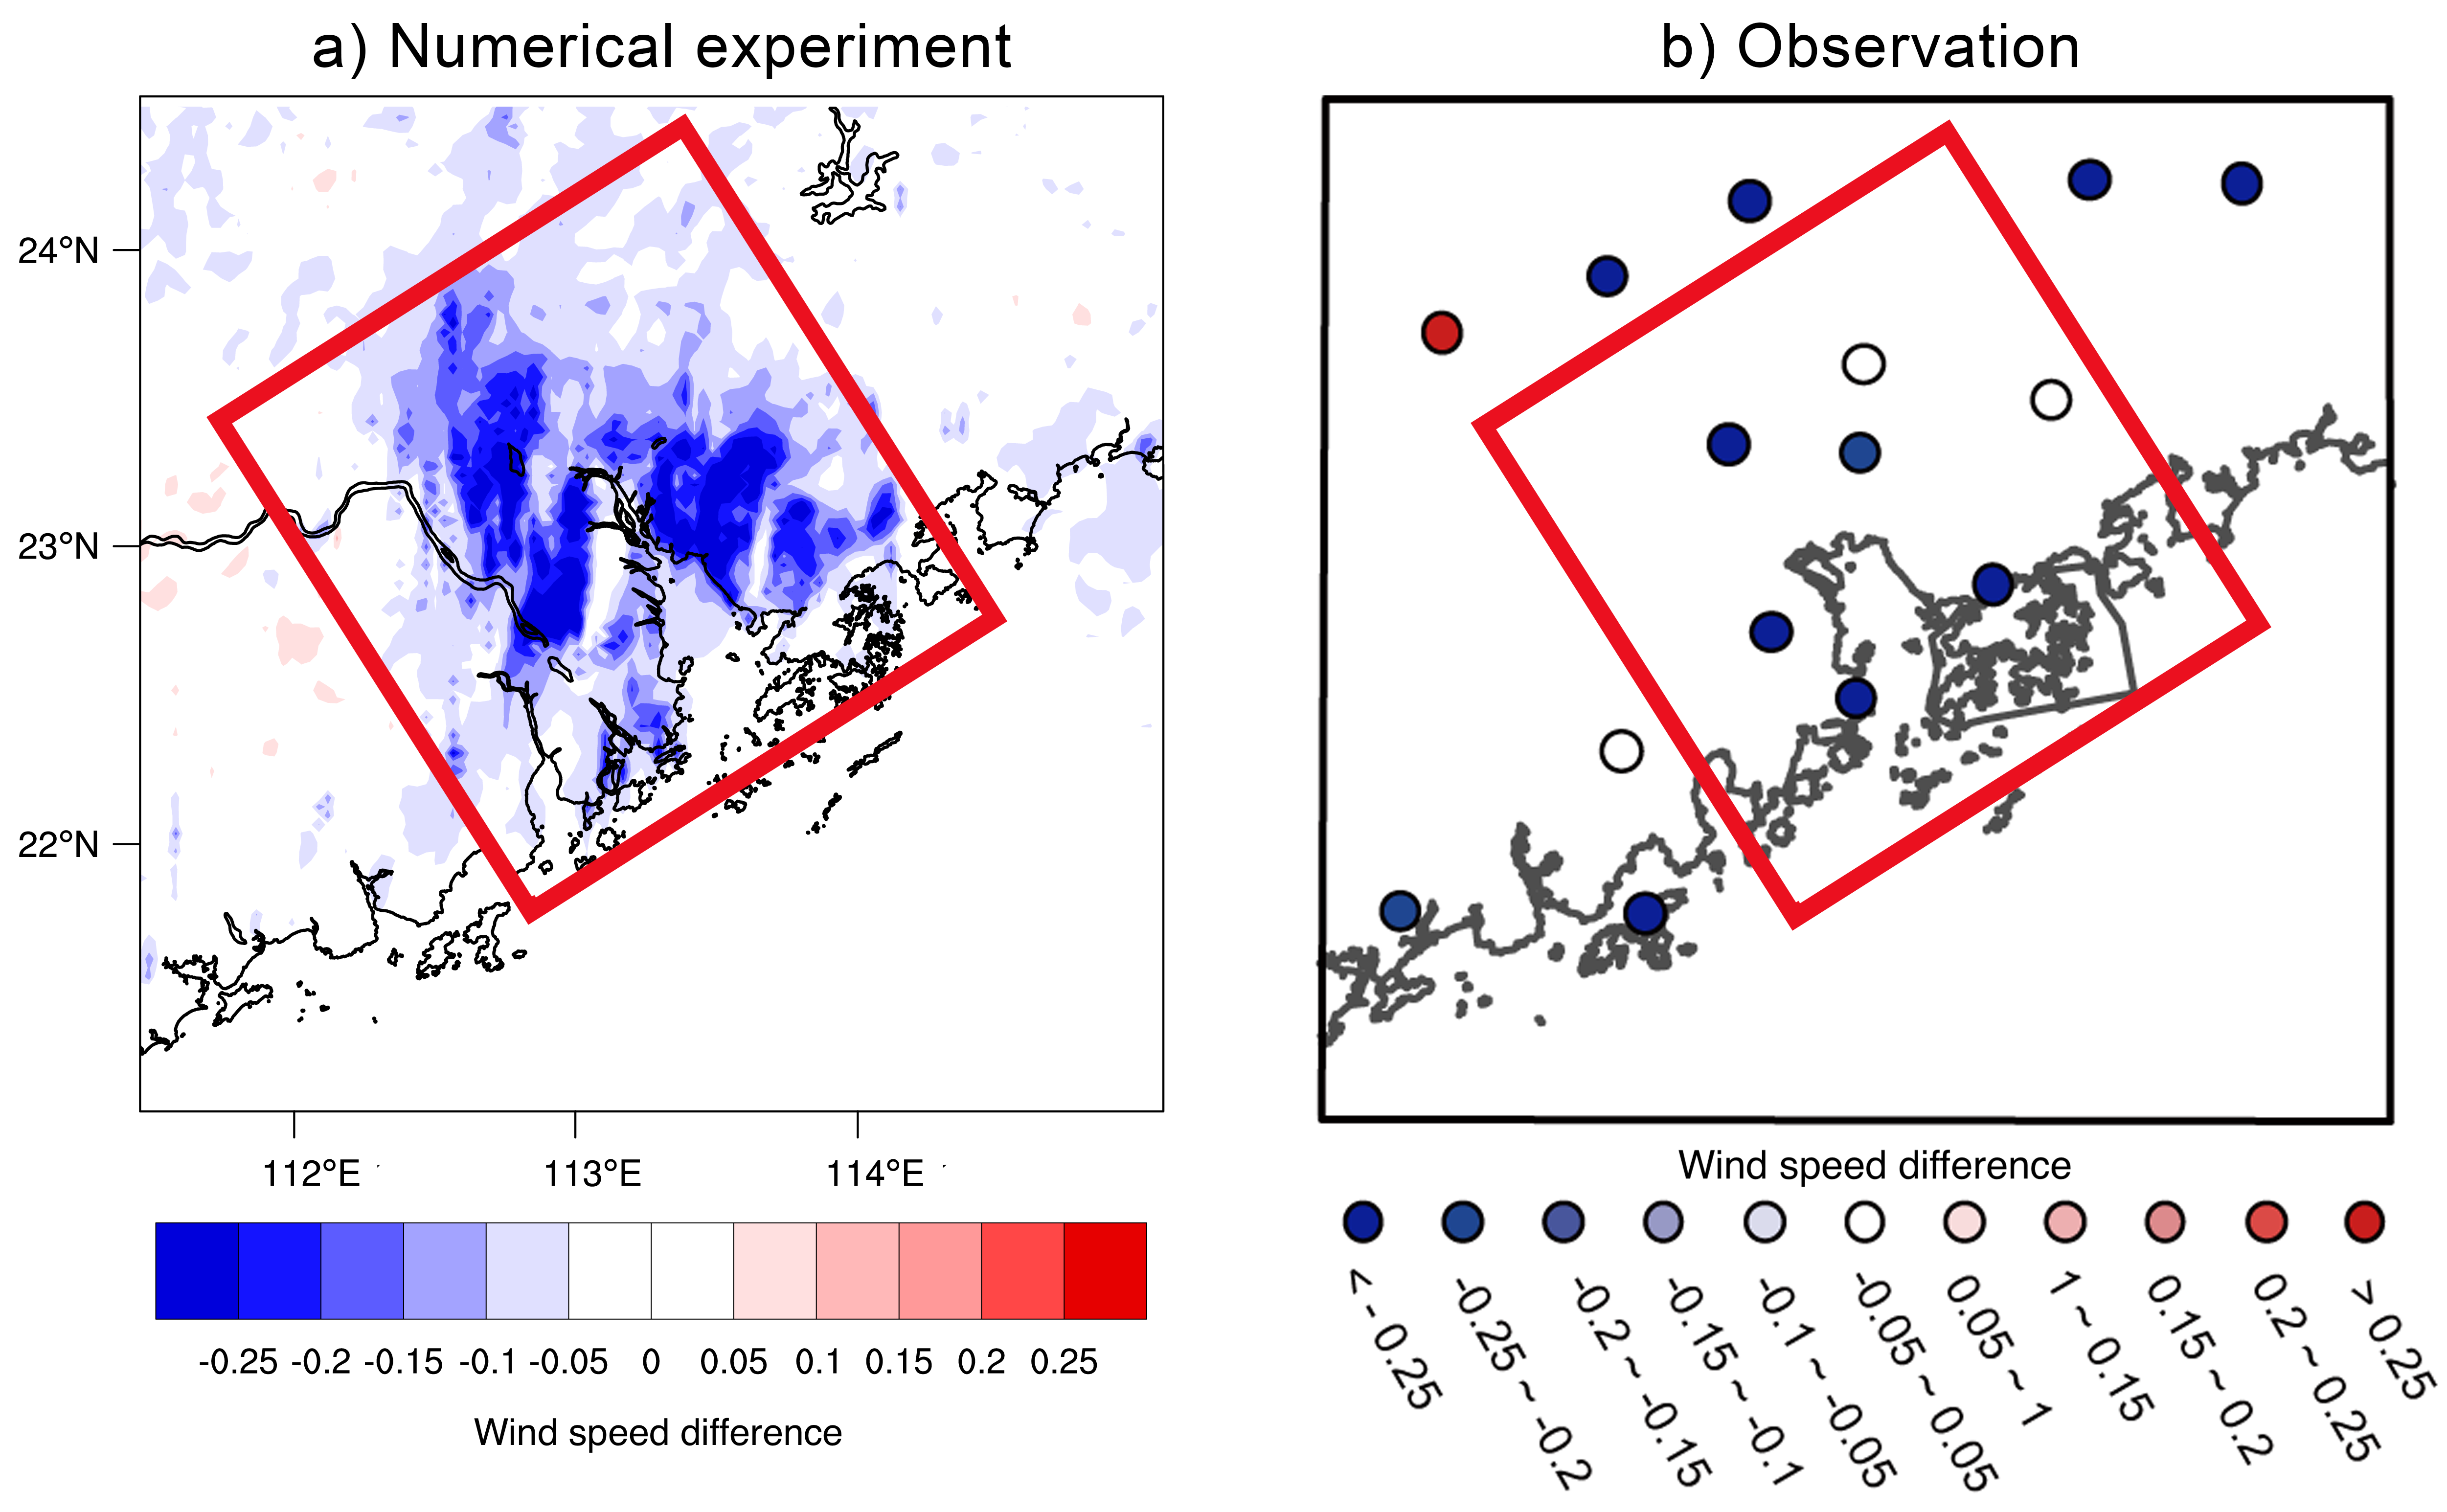
\includegraphics[width=0.9\textwidth]{珠江三角洲模拟结果与观测对比}
    \bicaption{ 珠江三角洲模拟与观测风速变化(变化率)。a)模拟结果,b)观测结果。}{Simulated and observed wind speed change in the Pearl River Delta (in $changing ~ rate$). a)Simulation, b)Observation.}
    \label{fig:wrfvsobs}
\end{figure}

将模拟\ref{sim:1.2} 与模拟\ref{sim:1.1} 的模拟结果相减,得到城市建设面积变化对于地表风速的影响。发现相对20世纪70年代末,珠江三角洲在2015年城市化状况下风速显著偏小,城市群所在区域风速差可达 1 $m ~ s^{-1}$以上。同时,城市群下风向地区风速也表现出偏小,6月珠江三角洲盛行偏南风,城市群北部有风速偏小区域;12月珠江三角洲盛行偏北风,城市群南部有风速偏小区域(图 \ref{fig:urbanizationonwind})。将两个月模拟结果平均,并差值到6个观测站点(图 \ref{fig:wrfvsobs} b) 红框内),得到风速平均减小了11.6\%,相比之下,观测风速在1979-2016平均减小了33.4\%,由此可得城市化对于风速减小的贡献达到35\%(图 \ref{fig:wrfvsobs})。此外,城市化对于风速的影响主要体现在大风,2 $m ~ s^{-1}$以下风速变化很小(图 \ref{fig:windPDF})。

\begin{figure}[!htbp]
    \centering
    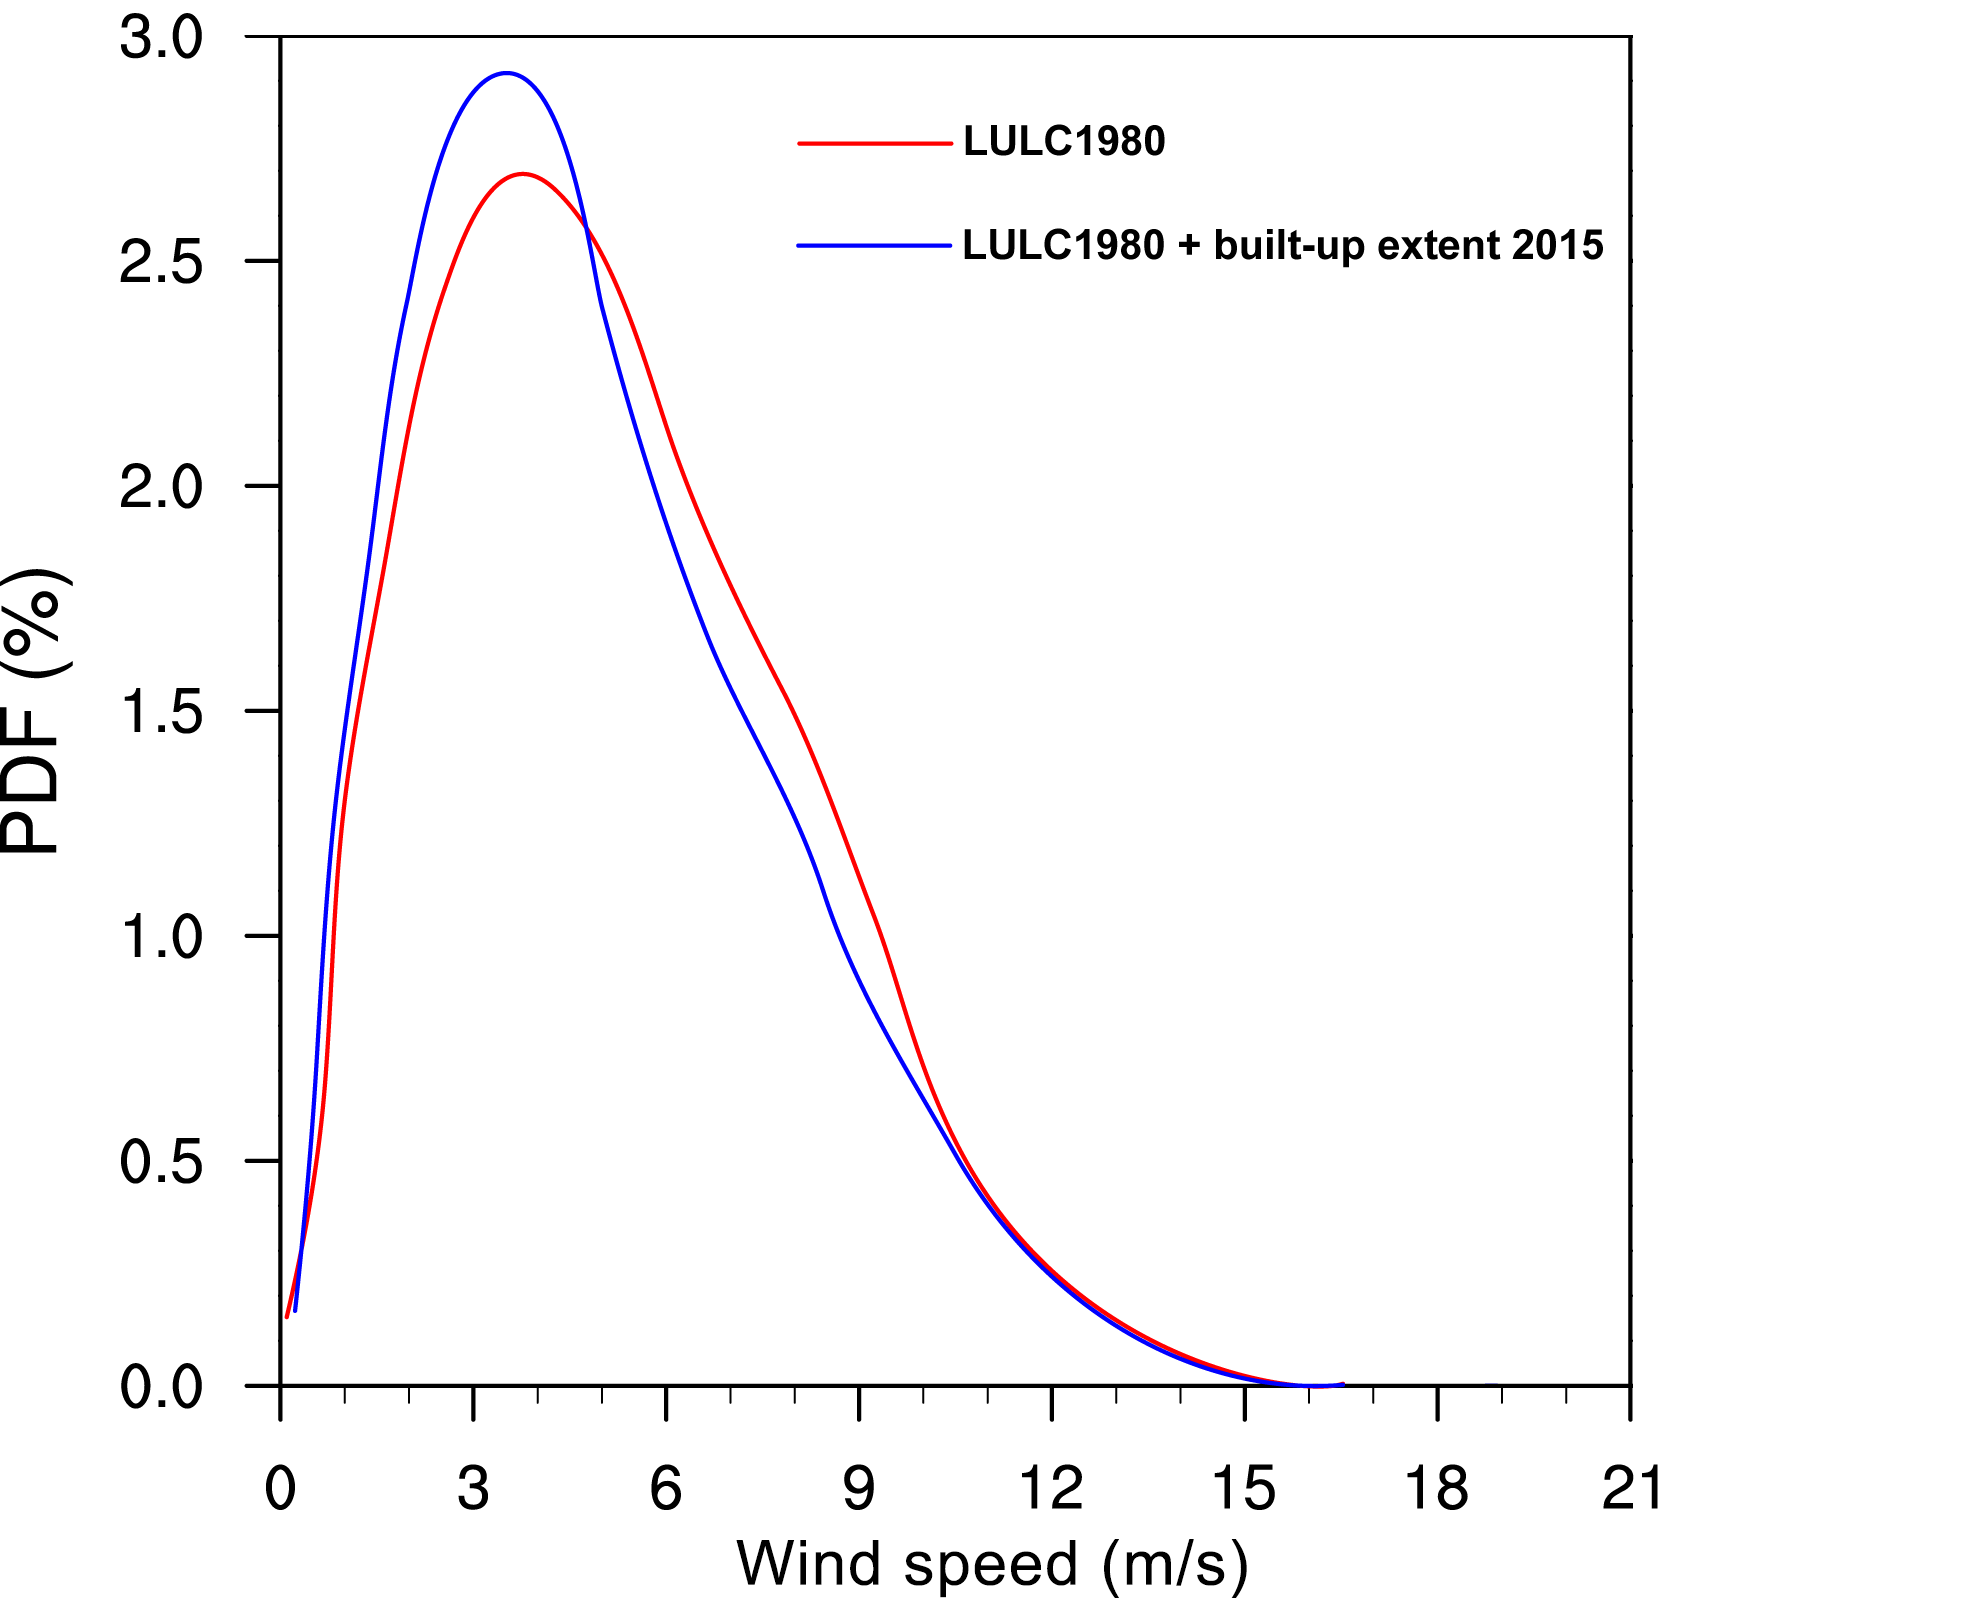
\includegraphics[width=0.7\textwidth]{城市化对风速概率密度分布的影响}
    \bicaption{ 珠江三角洲20世纪70年代末与2015年城市化状况下风速概率密度分布。红色(蓝色)实线为使用20世纪70年代末城市化状况(2015年城市化状况)的模拟结果。}{Probability distribution function of wind speed in the Pearl River Delta under the built-up condition in late 1970s and 2015. Red (Blue) line is the simulation result using built-up condition in late 1970s (2015).}
    \label{fig:windPDF}
\end{figure}

\section{植被变化的影响}

\subsection{基于NDVI和风速观测数据的统计学分析}

使用GIMMS NDVI 3g观测站点周围3 $ \times$ 3(\textasciitilde 25 $\times$ 25km)北半球植被生长期(4-9月)平均计算得到1982-2015年NDVI趋势,发现亚洲和欧洲的大部分区域NDVI有显著增加,表明植被有明显增加,相比之下,北美洲NDVI无明显趋势(图 \ref{fig:NDVItrend})。将NDVI趋势与风速趋势对比,没有发现有明显的相关关系,原因可能是草地等低矮植被的变化对10 m风速无明显影响,而林地等高大植被变化才能够对10 m风速产生影响。选取林地覆盖面积超过90\%的芬兰,且其在2001-2016年间有超过95\%的植被变化来自林地变化(图 \ref{fig:Finlandvegetation}),发现NDVI趋势与风速趋势呈显著负相关(p < 0.05)(图 \ref{fig:FinlandwindvsNDVI}),表明植被(主要是林地)增加的区域风速趋向于减小。

\begin{figure}[!htbp]
    \centering
    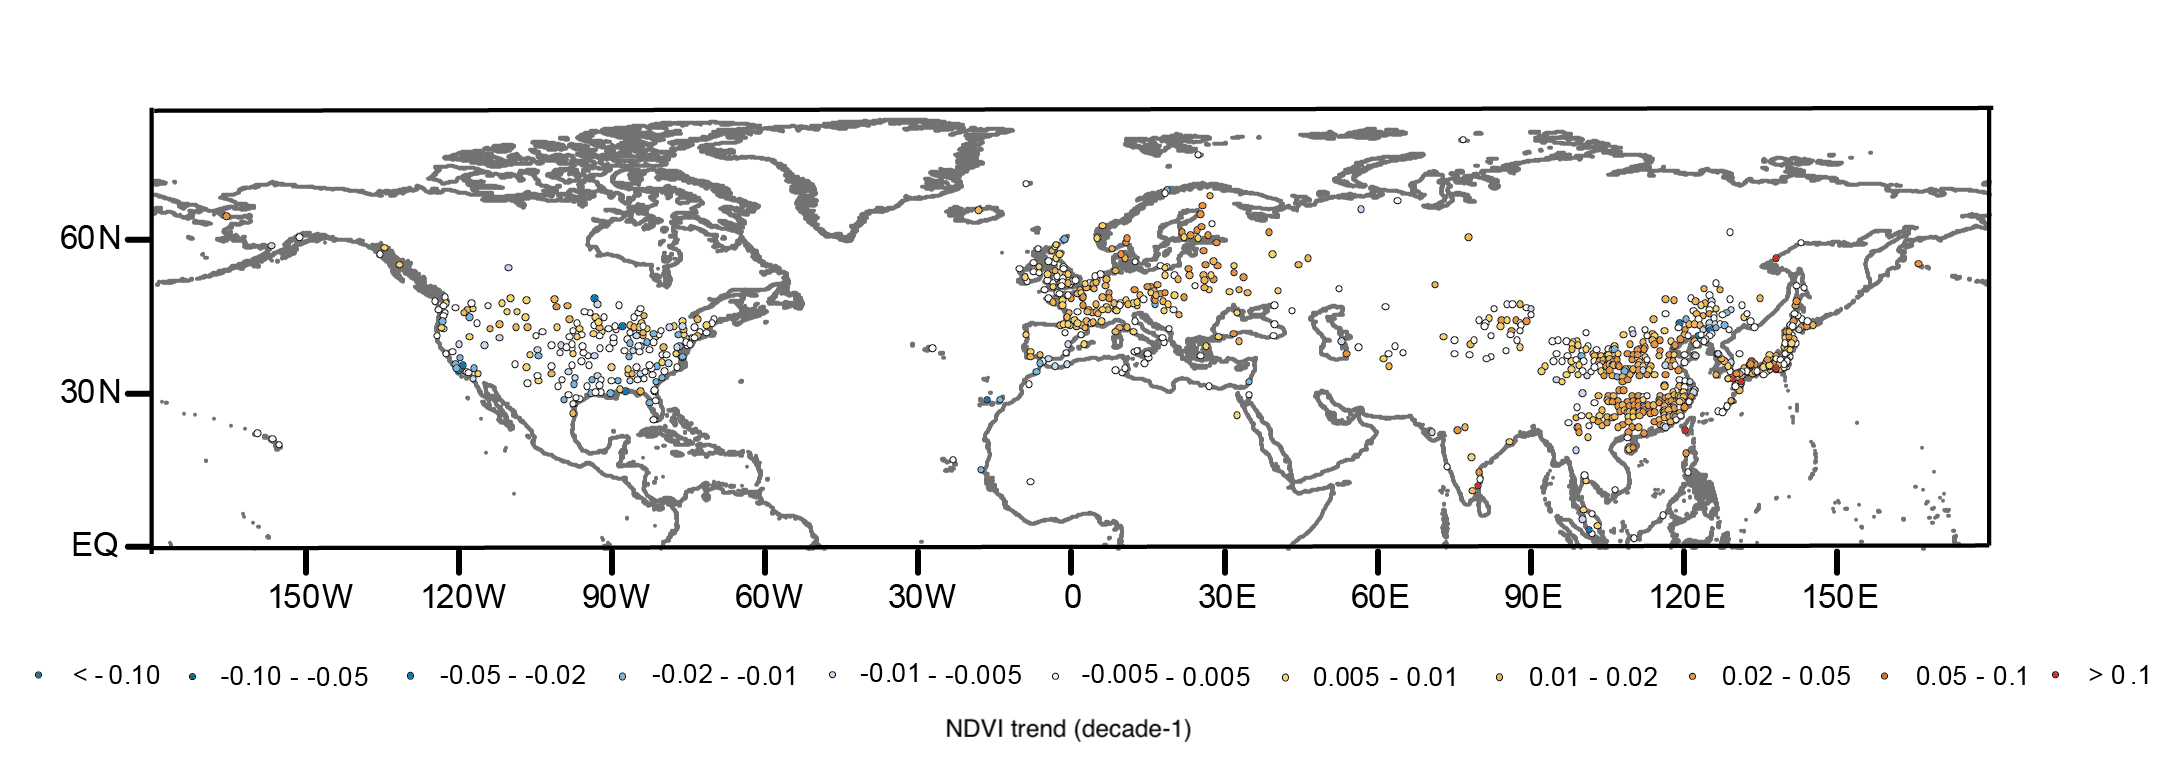
\includegraphics[width=1 \textwidth]{NDVI趋势}
    \bicaption{北半球植被生长季NDVI趋势( 每十年)}{Growing season NDVI trend over the Northern Hemisphere (in $decade^{-1}$).}
        \label{fig:NDVItrend}
\end{figure}

\begin{figure}[!htbp]
    \centering
    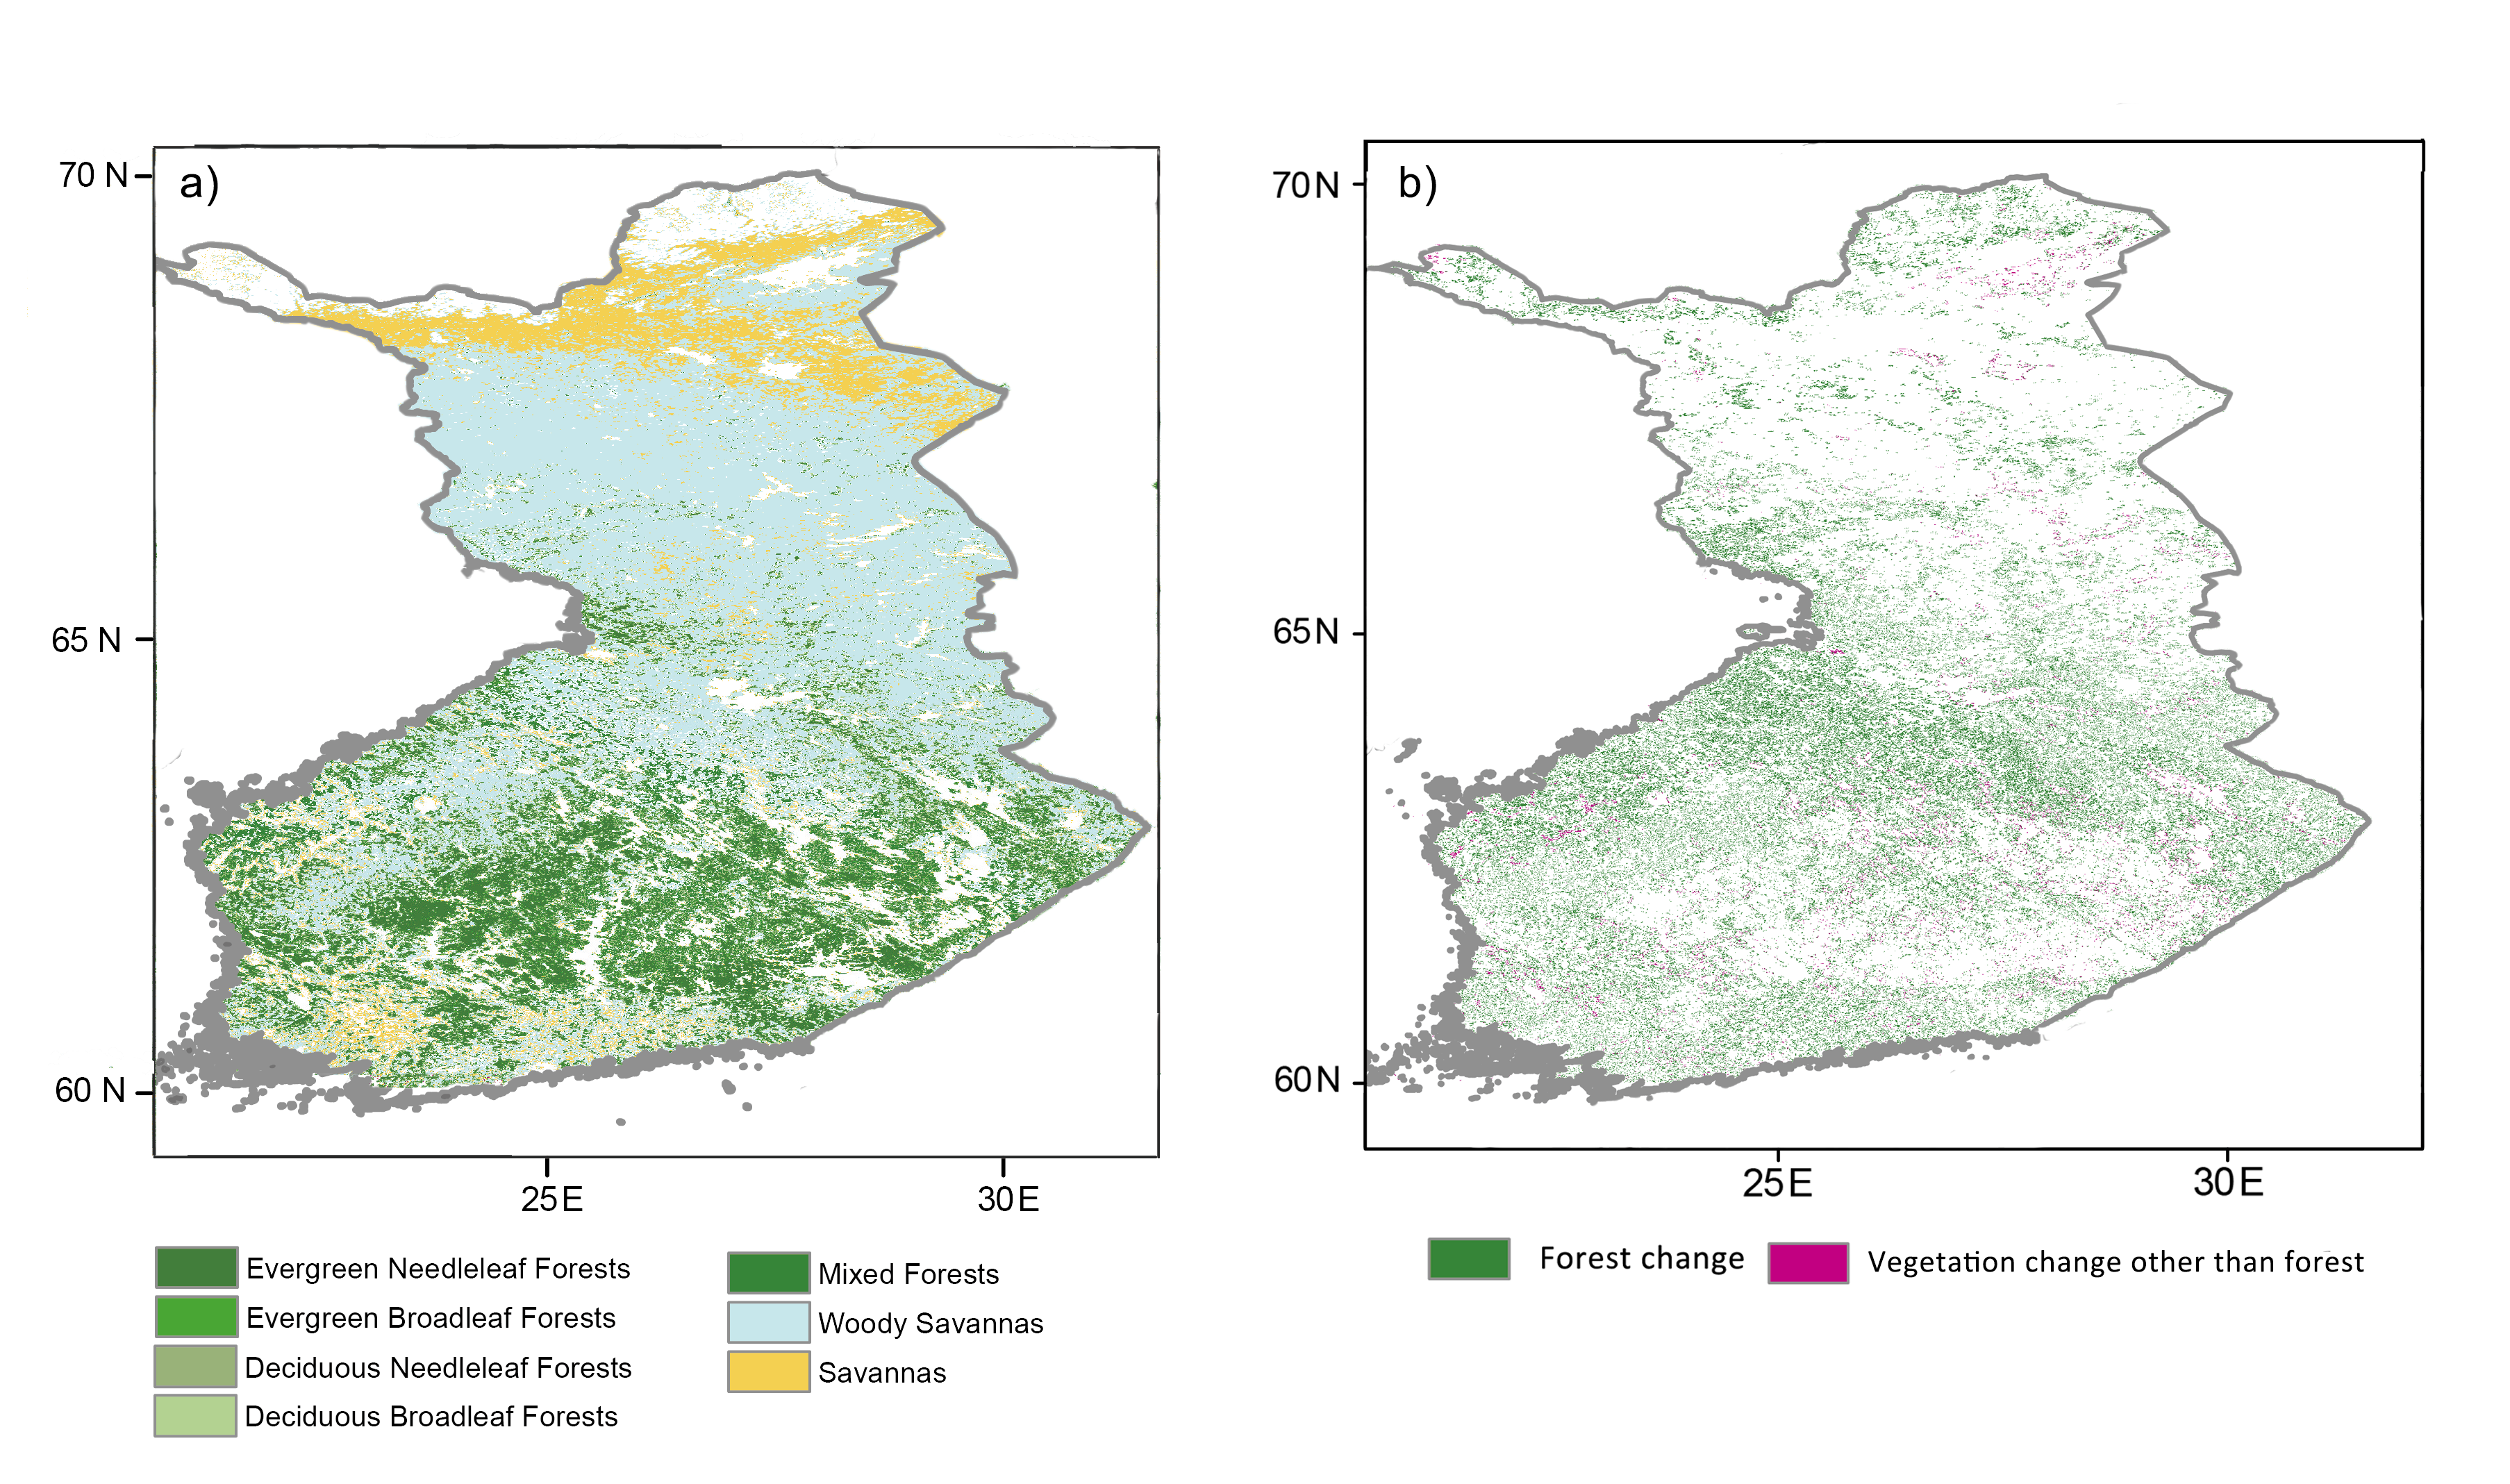
\includegraphics[width=0.9 \textwidth]{芬兰植被分布与变化}
    \bicaption{芬兰植被分布与变化。a)芬兰2001年林地分布,b)芬兰2016相对2001植被变化,绿色为林地变化,红色为除林地外其他植被变化。}{Spatial distribution and temporal change of vegetation in Finland. a)Spatial distribution in 2000, b)Change from 2001 to 2016, green denotes woodland change, red denotes vegetation change other than woodland.}
        \label{fig:Finlandvegetation}
\end{figure}

\begin{figure}[!t]
    \centering
    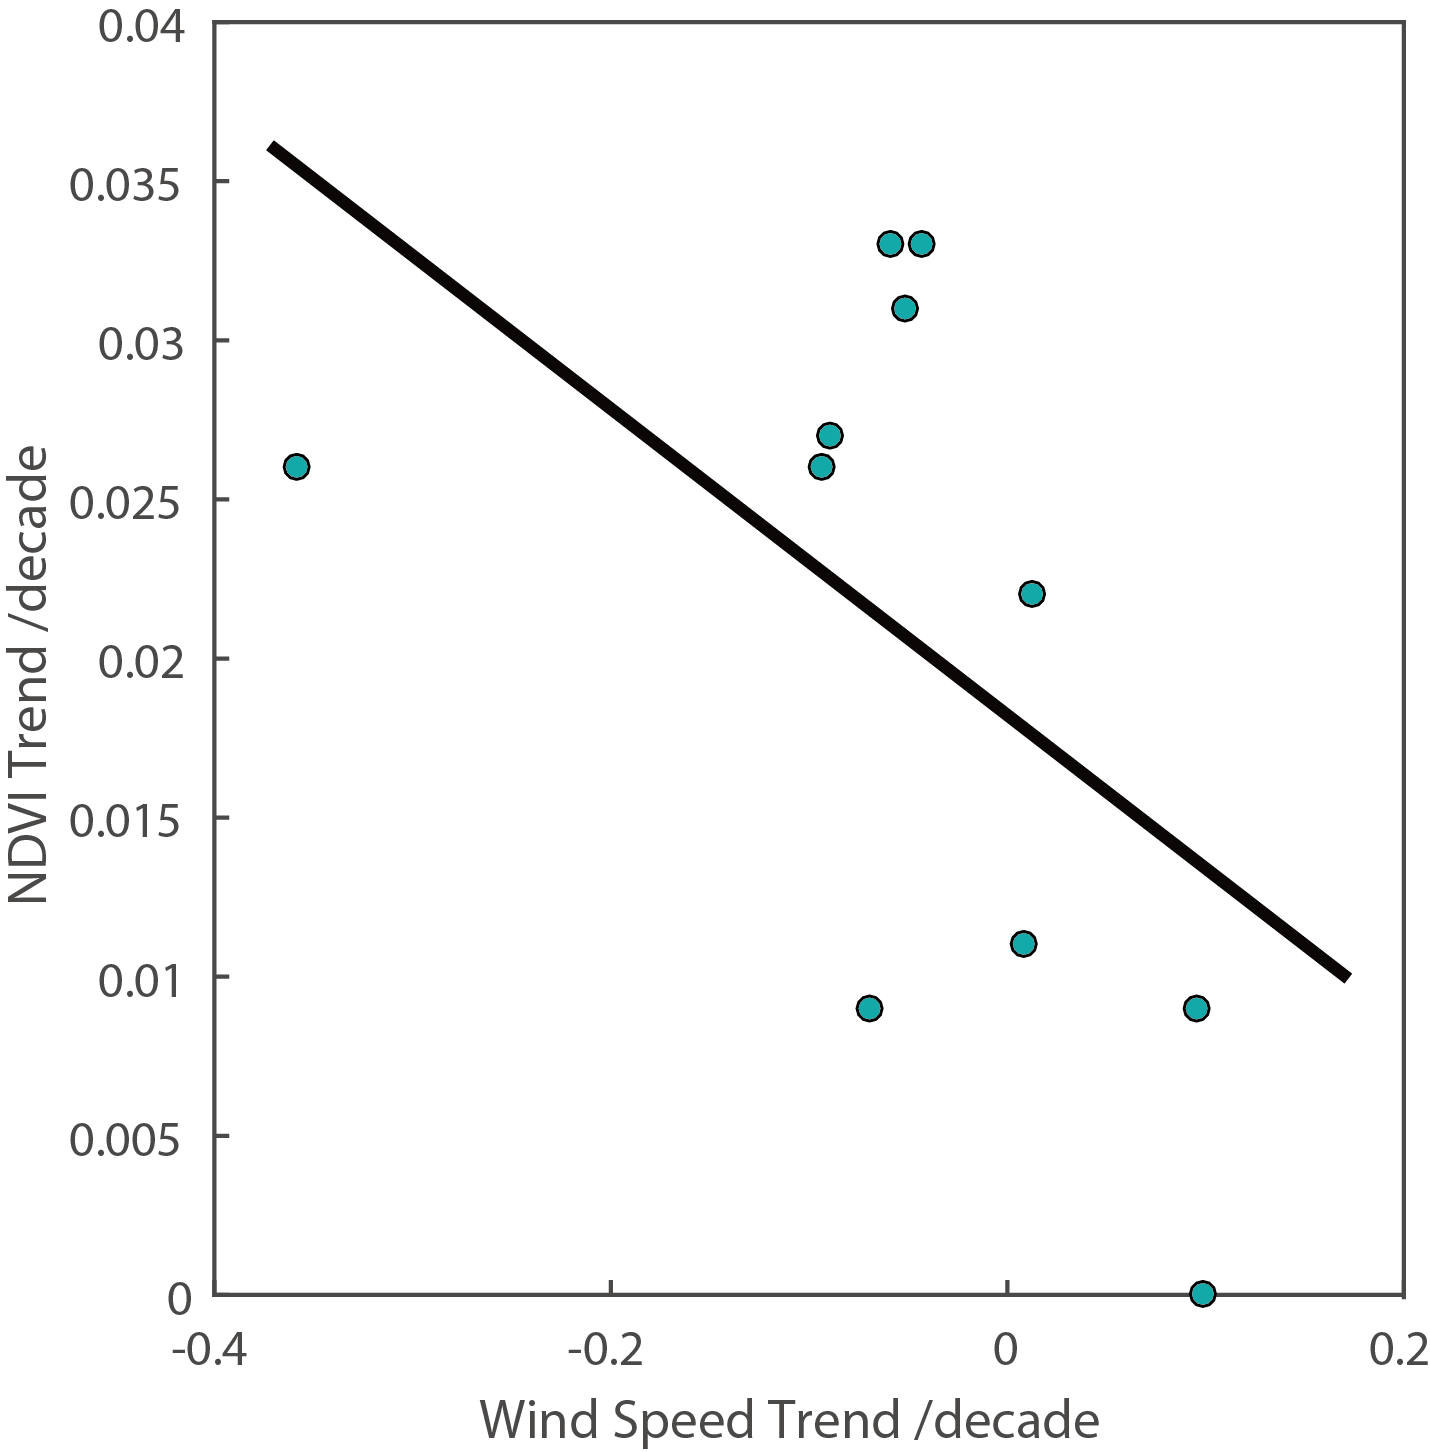
\includegraphics[width=0.5 \textwidth]{ndvi与风速变化}
    \bicaption{芬兰站点风速趋势与附近NDVI趋势}{Wind speed trend and NDVI trend nearby in Finland.}
        \label{fig:FinlandwindvsNDVI}
\end{figure}

\subsection{数值试验}

使用WRF-ARW 4.0进行数值试验进一步验证植被与风速变化的关系,选择芬兰植被变化更为明显同时也是大部分观测站点所在的南芬兰作为模拟区域(图 \ref{fig:Finlandstations})。将模式设置为四层双向嵌套,空间分辨率分别为30km、10km、3.3km和1.1km(图 \ref{fig:Finmodeldomain}),垂直包含40个层次,其中边界层内(1km高度以下)10个层次;时间步长为100 s;微物理参数化方案为WRF Single-Moment 6-class scheme;积云参数化方案为Grell 3D,在较高分辨率的两层网格关闭积云参数化;云量使用Xu-Randall method;长波辐射参数化方案为RRTM scheme,短波辐射参数化方案为Dudhia scheme;边界层采用BouLac PBL,地面层采用Eta similarity,陆面模式选择Noah-MP。

\begin{figure}[!hbtp]
    \centering
    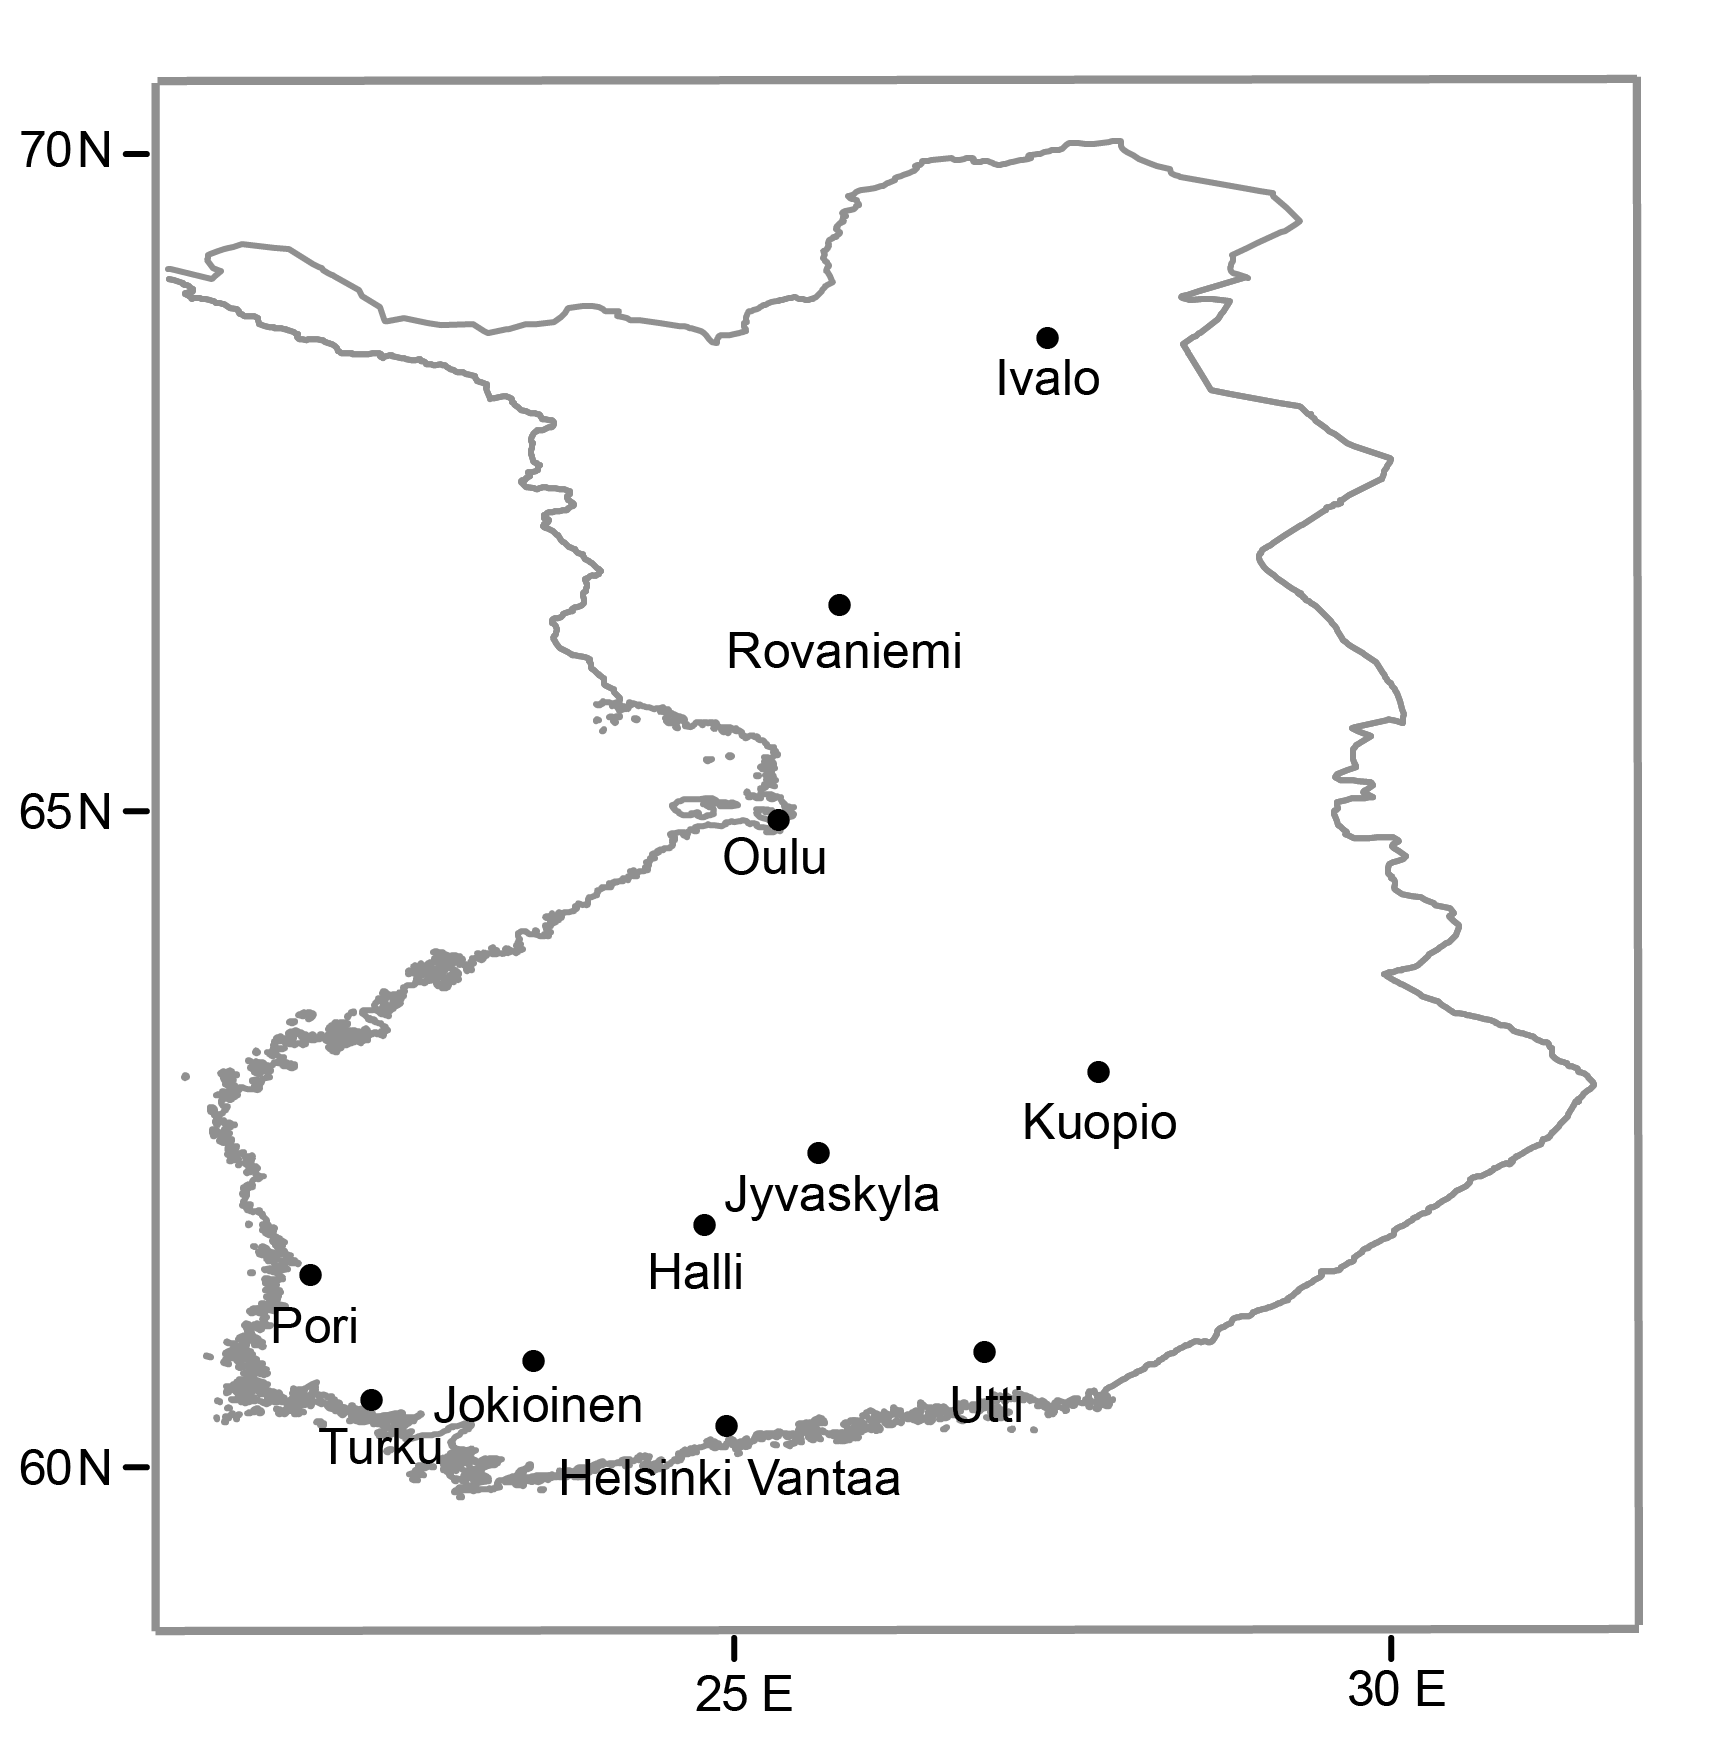
\includegraphics[width=0.6 \textwidth]{芬兰站点分布}
    \bicaption{芬兰站点分布}{Locations of observation stations in Finland.}
        \label{fig:Finlandstations}
\end{figure}

\begin{figure}[!hbtp]
    \centering
    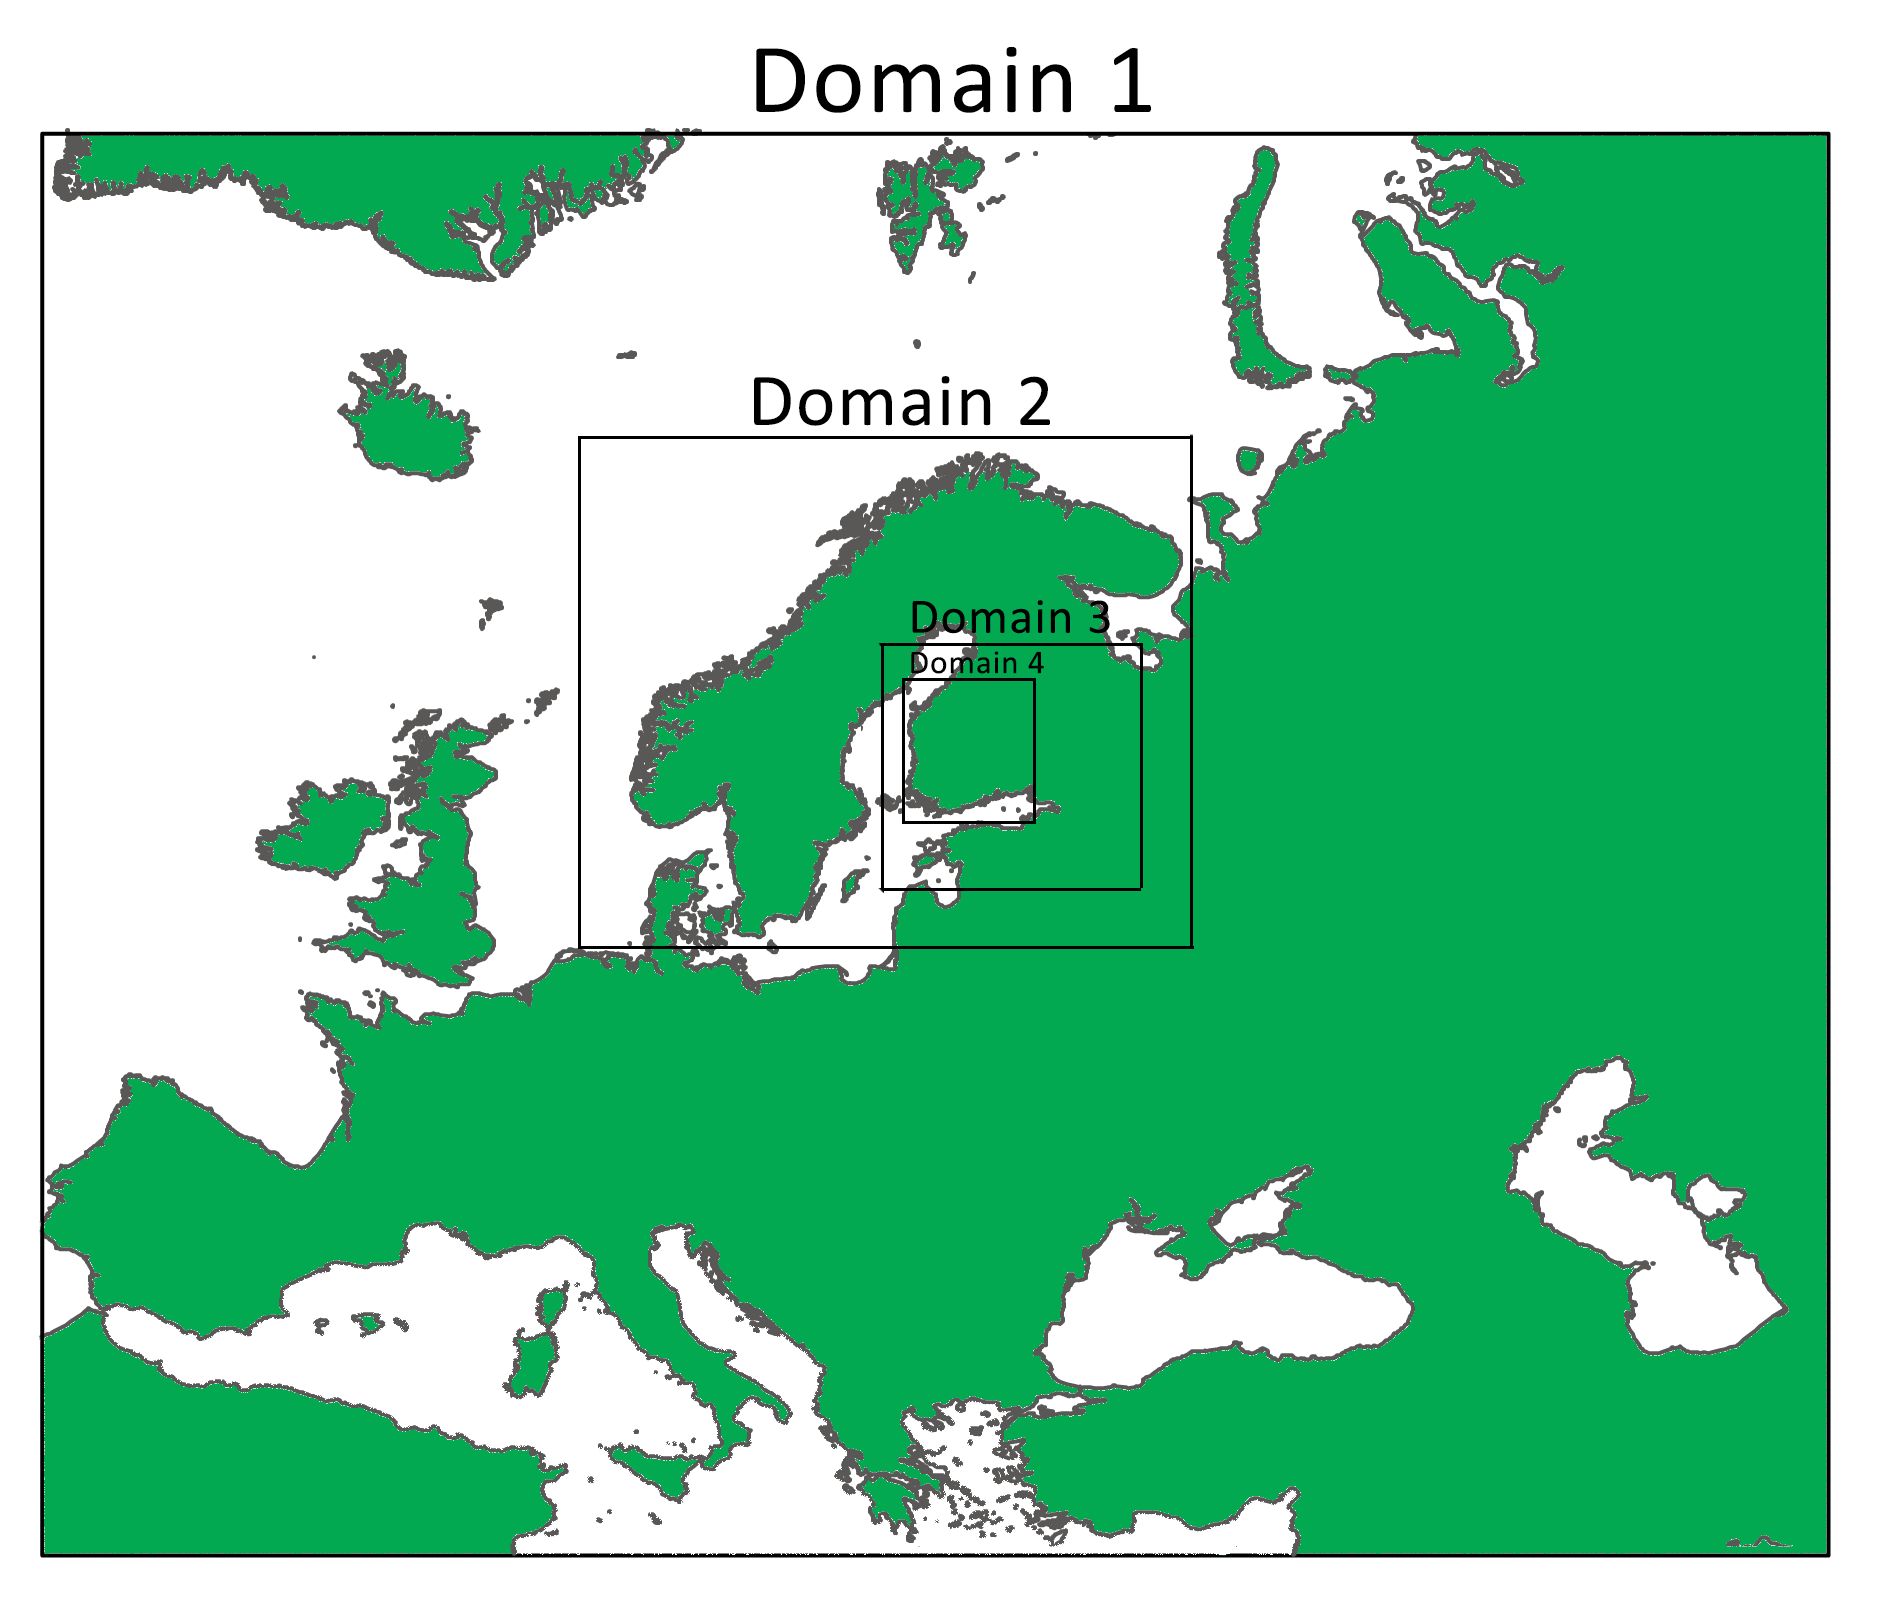
\includegraphics[width=0.8 \textwidth]{模拟区域2}
    \bicaption{模拟区域}{Model simulation domains}
        \label{fig:Finmodeldomain}
\end{figure}

采用以上模式设置进行两组模拟,分别为:

\begin{enumerate}

\item \label{sim:2.1} 以南芬兰地区2001年土地利用类型(MODIS12Q1)作为下边界条件进行模拟。

\item \label{sim:2.2} 以南芬兰地区2001年土地利用类型叠加2016相对2001年南芬兰地区林地变化作为下边界条件进行模拟。

\end{enumerate}

对以上两组模拟,气象场采用FNL2001年1月和2001年6月(分别代表植被非生长季节和生长季节)1$\times$ 1度6小时分辨率物理量场。

使用模拟\ref{sim:2.1}进行模式性能评估,南芬兰地区观测站信息参见表 \ref{tab:Finlandstationinfo},表中除Oulu、Rovaniemi、Ivalo外,其余站点均分布在南芬兰。对比模拟与观测结果,与本章/ref{sec:urbanimpact}节类似,模拟风速大于观测风速,但二者相关系数较高,表明模拟能够较好的抓住风速随时间的变化,RMSD也较低,总体来看模式模拟效果良好。

\begin{table}[!htbp]
    \bicaption{南芬兰站点信息及模式性能评估结果}{Description of observation stations in the southern Finland and model validation results}
    \label{tab:Finlandstationinfo}
    \centering
    \small% fontsize
    \setlength{\tabcolsep}{5 pt}% column separation
    \renewcommand{\arraystretch}{1.0}%row space 
    \begin{tabular}{lccccccc}
        \hline
        站名 & 站号 & 纬度 & 经度 & 海拔(m)&  \multicolumn{3}{c}{10 m 风速} \\
         & & & & & 均值($m ~ s^{-1}$)$^*$ &  相关系数 $^ {**}$ & RMSD \\
        %\cline{2-9}% partial hline from column i to column j
        \hline
        Pori & 29520 & 61.47 & 21.8 & 13.4 & 5.4(-1.4) & \textbf{0.38} & 1.35 \\
        Turku & 29720 & 60.52 & 22.27 & 49.1 & 5.0(-1.7) & 0.26 & 1.57 \\
        Jokioinen & 29630 & 60.82 & 23.50 & 103.0 & 4.8(-1.8) & 0.04 & 1.41 \\
        Helsinki & 29740 & 60.32 & 24.97 & 54.6 & 4.5(-0.6) & \textbf{0.34} & 1.27 \\
        Vantaa & & & & & & \\
        Halli & 29450 & 61.80 & 24.80 & 146.0 & 4.6(-1.5) & \textbf{0.36} & 1.34 \\
        Jyvaskyla & 29350 & 62.40 & 25.67 & 139.9 & 4.5(-1.1) & 0.27 & 1.43 \\
        Utti & 29660 & 60.88 & 26.93 & 103.3 & 4.0(-0.8) & \textbf{0.34} & 1.33 \\
        Kuopio & 29170 & 63.02 & 27.80 & 98.5 & 5.2(-1.9) & \textbf{0.42} & 0.99 \\ 
        \hline
    \end{tabular}
    \vspace*{3ex}
    \begin{minipage}{0.9\textwidth}% choose width suitably
    注:$^*$ 括号外数值为模拟结果,括号内为观测减去模拟。\\ 
    $^{**}$ 加粗的数值代表 p < 0.01。r = 0.33 对应 p = 0.01, r = 0.25 对应 p = 0.05。
    \end{minipage}
\end{table}


将模拟\ref{sim:2.2}与\ref{sim:2.1}相减,得到林地变化对于风速的影响。由林地变化造成的对风速影响中,主要的作用是风速减小(图 \ref{fig:woodlandonwind}),考虑到林地变化中的超过70\%是增加(图(芬兰林地变化)),得到这种模拟结果非常合理。1月林地变化对于风速变化的影响明显小于7月,因而1月很多落叶林地变得光秃,对风速的影响变小。将两个月的模拟结果平均,计算归一化风速变化,差值到观测站点,得到南芬兰8个站点林地对风速影响平均为-2.5\%。假设林地变化与风速变化满足线性关系(即 $\Delta(woodland ~ area) = \alpha \Delta(wind ~ speed)$),并以NDVI代替林地变化,得到1979-2016林地变化对风速的影响在8个站点平均为-5.1\%,而观测风速的变化为-5.8\%,即林地变化可以解释南芬兰风速变化的87\%。

\begin{figure}[!t]
    \centering
    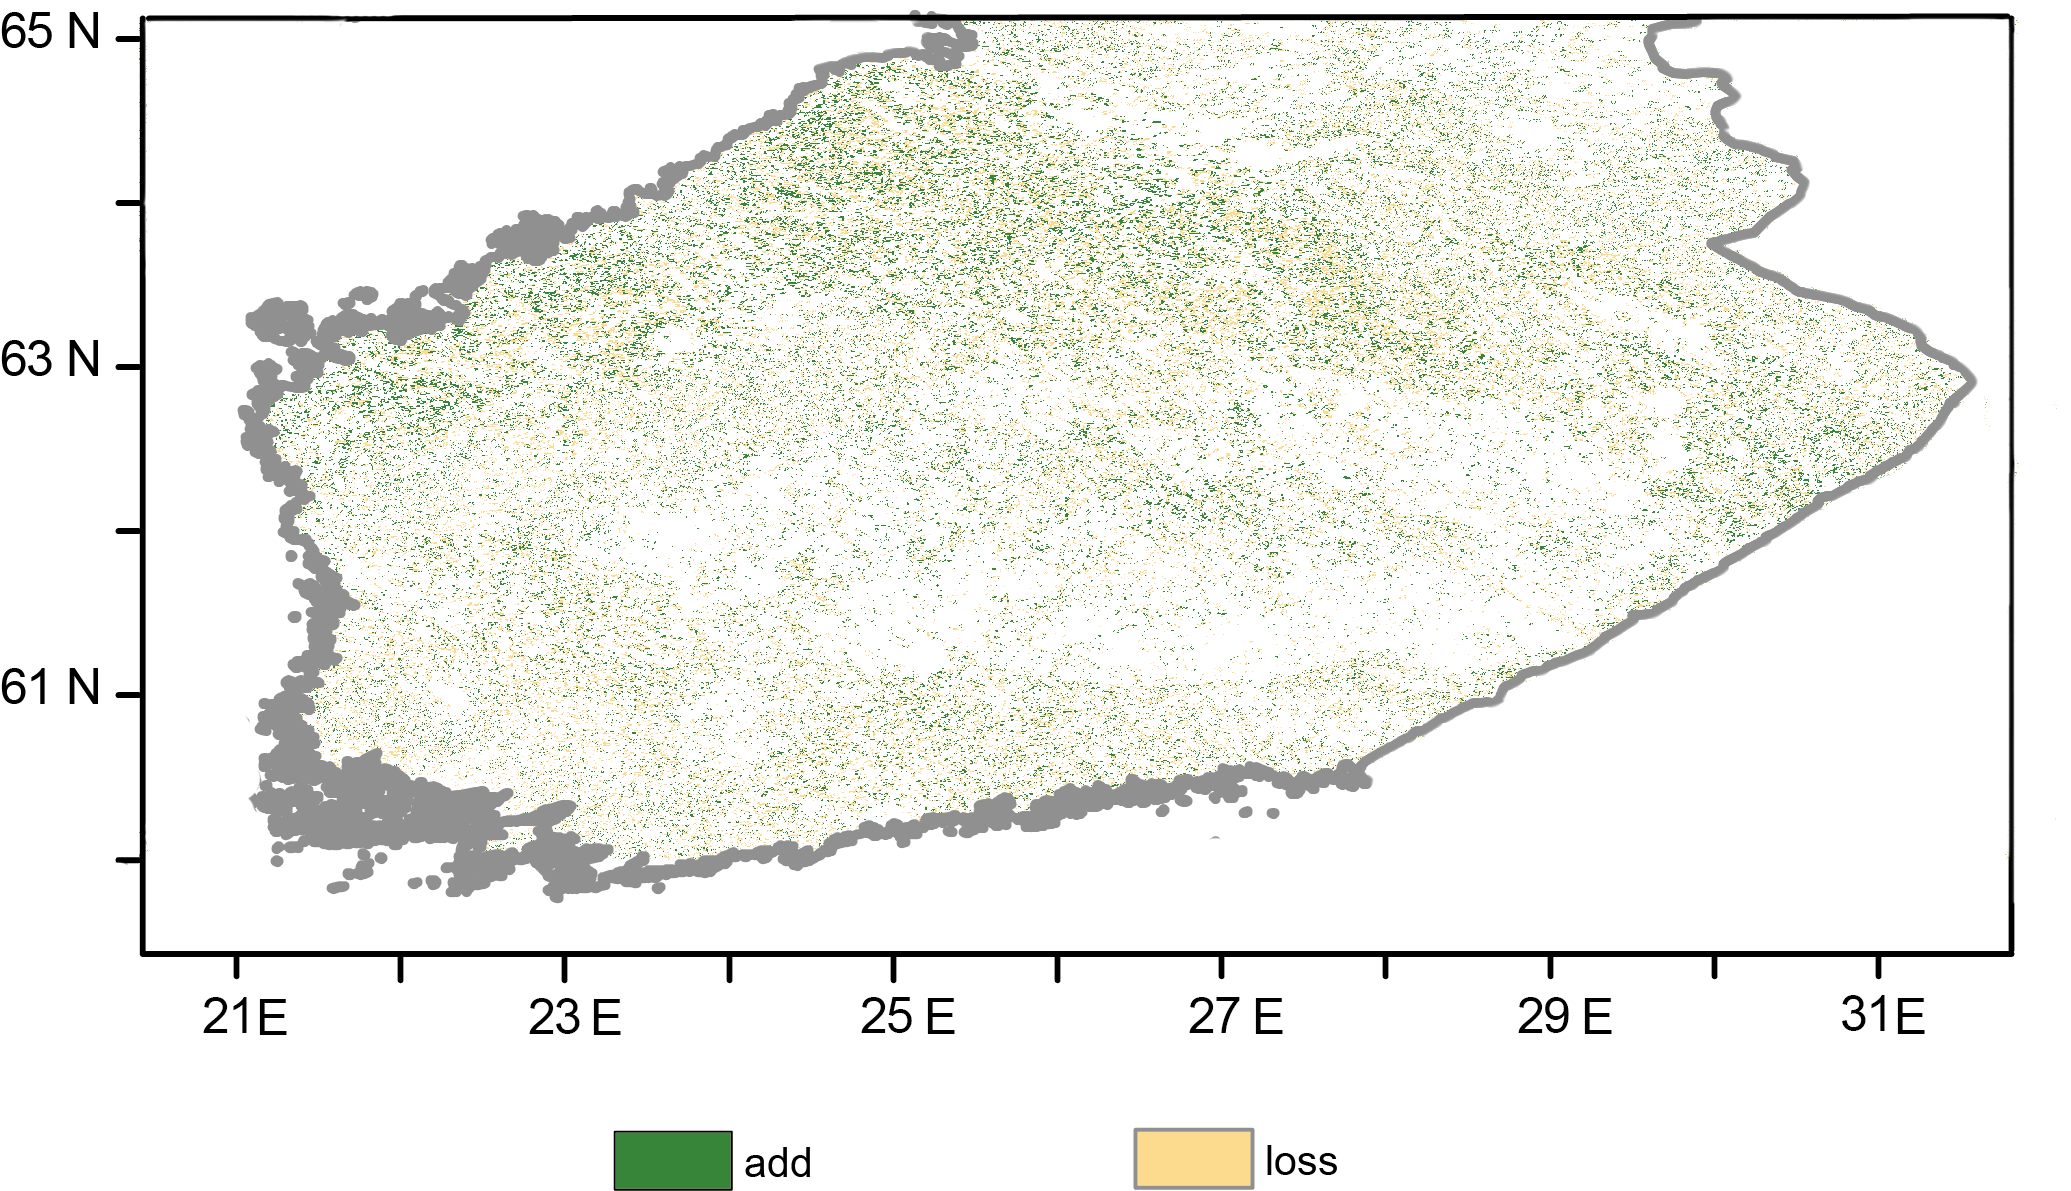
\includegraphics[width=0.6 \textwidth]{芬兰林地变化}
    \bicaption{南芬兰林地变化。绿色为增加,黄色为减少。}{Woodland change in southern Finland. Green color denotes add, yellow denotes lose.}
        \label{fig:Finlandwoodlandchange}
\end{figure}

\begin{figure}[!b]
    \centering
    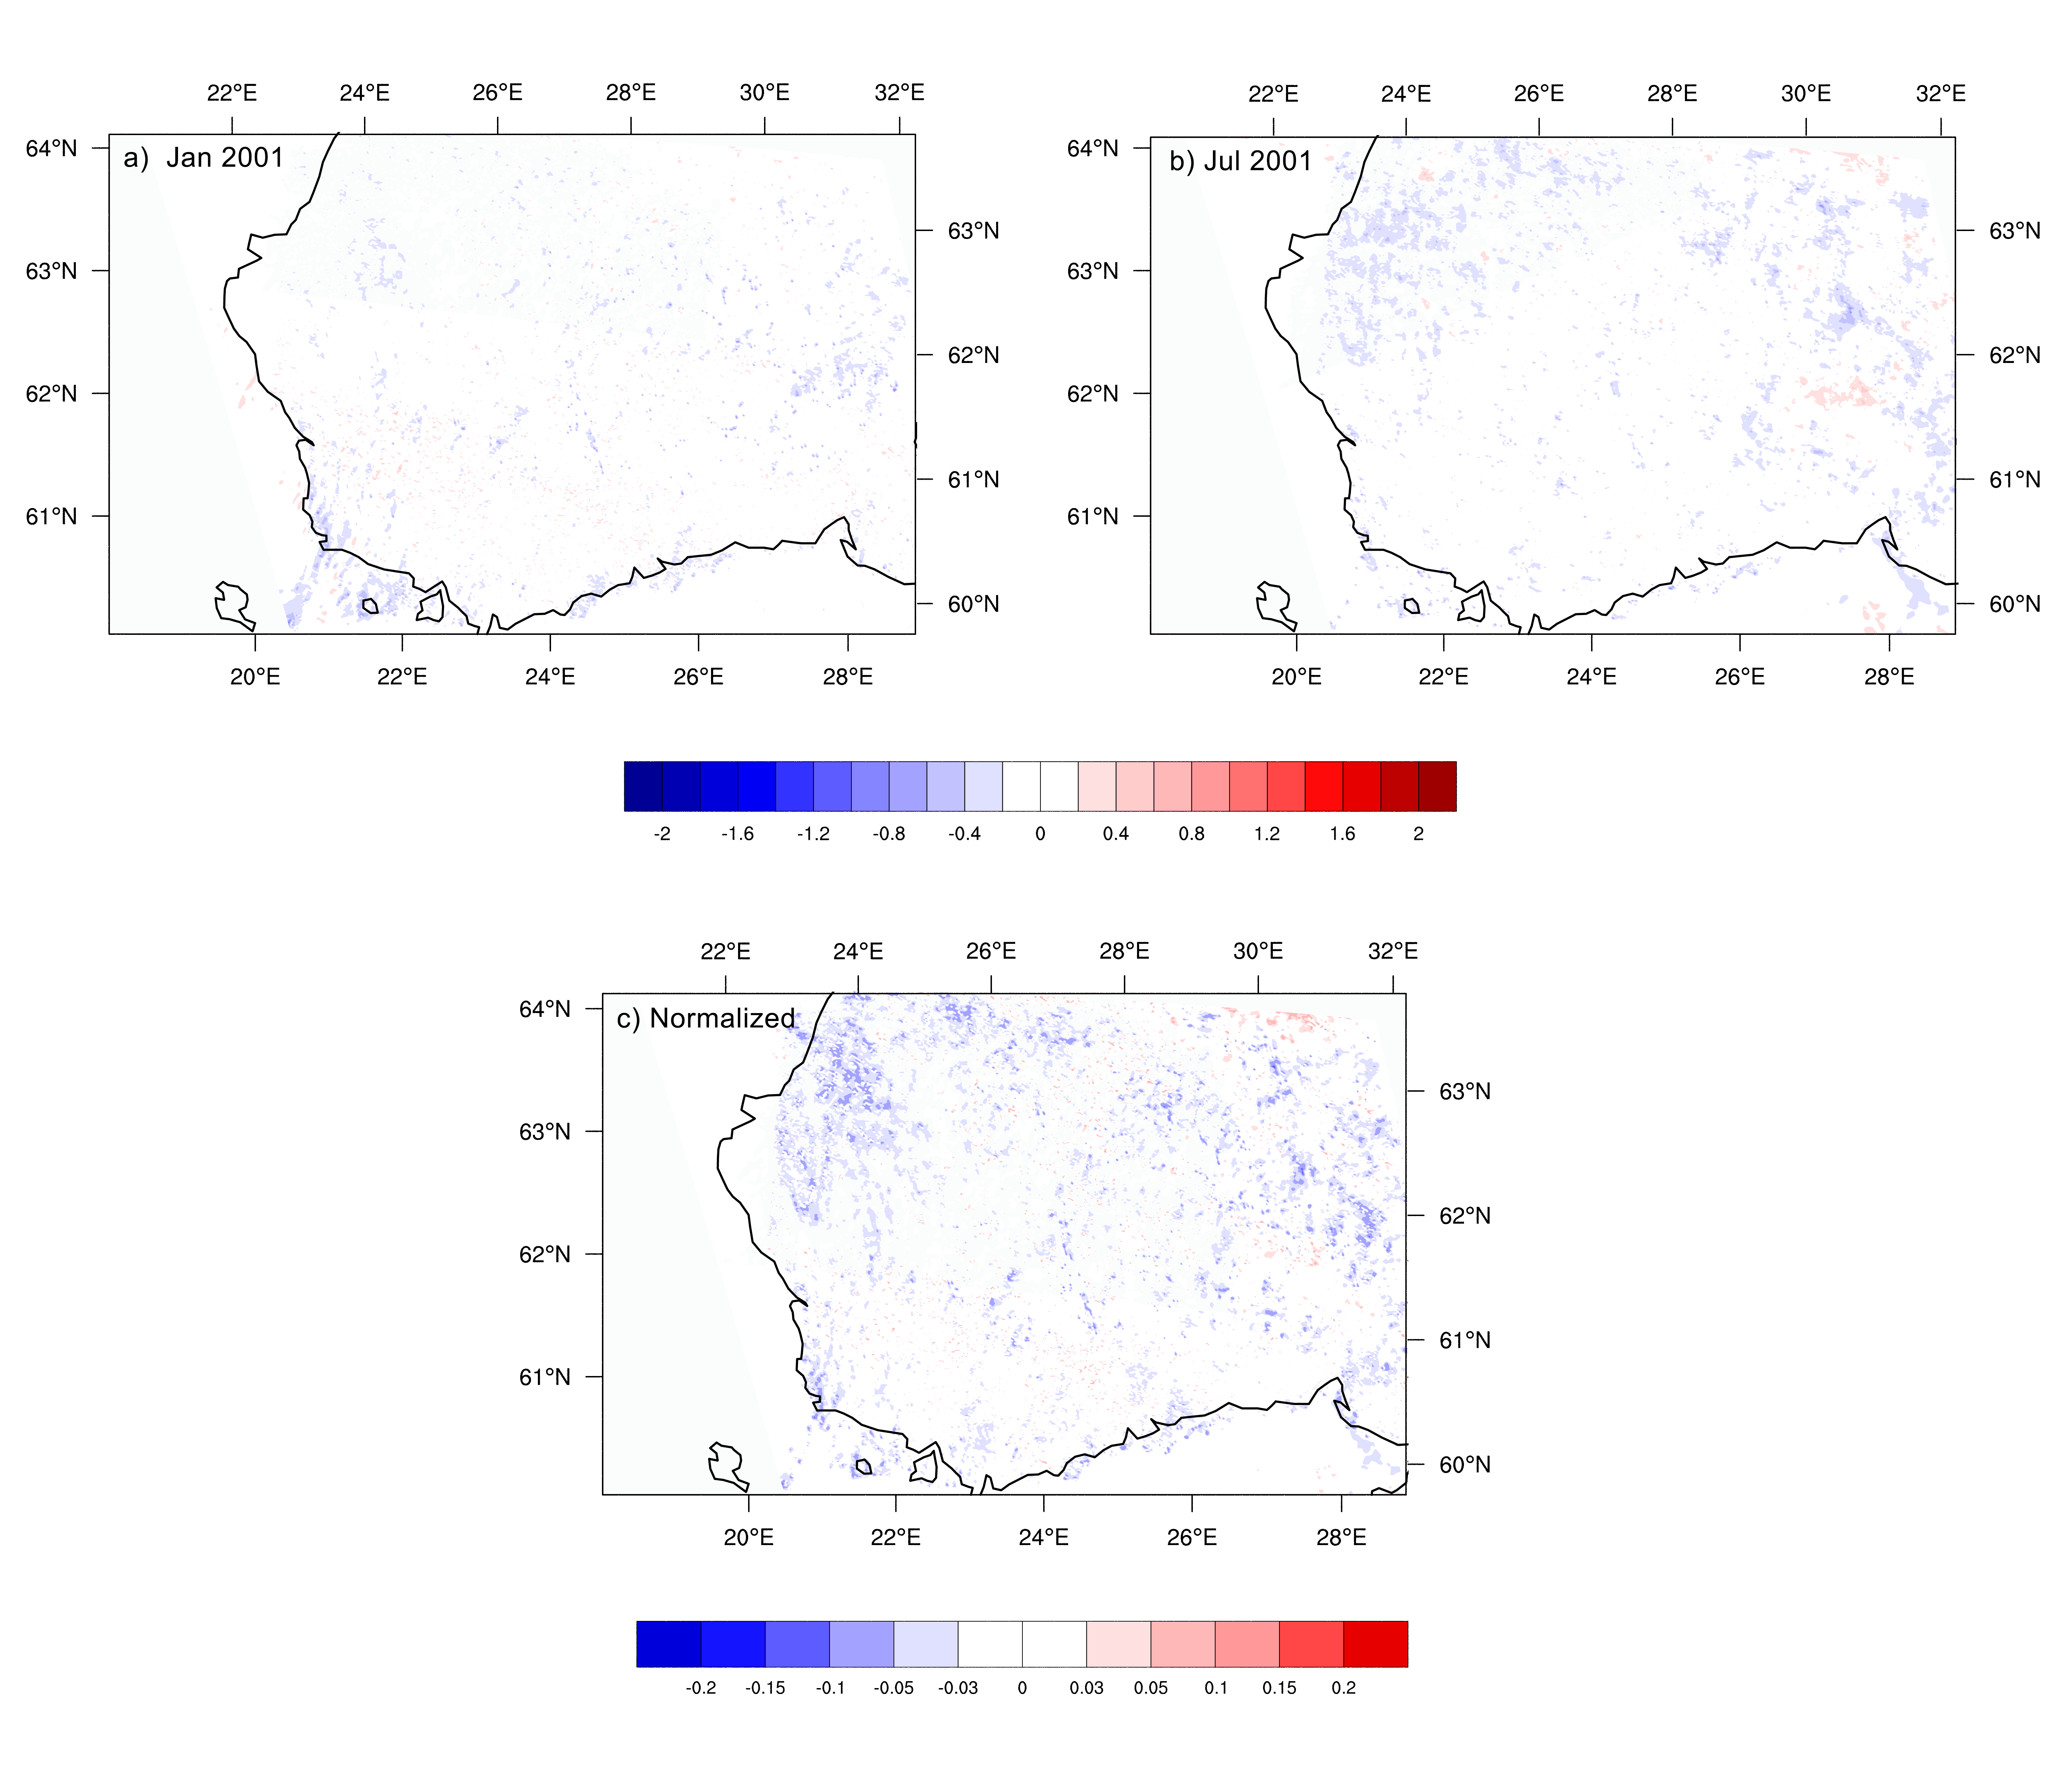
\includegraphics[width=1 \textwidth]{林地变化对地表风速的影响}
    \bicaption{林地变化对地表风速的影响。a)使用2001年1月气象场模拟结果($ m ~ s^{-1}$),b)使用2001年7月气象场模拟结果($ m ~ s^{-1}$),c)a和b模拟结果平均归一化的结果。}{Impact of woodland change on surface wind speed. a)Simulation with January 2001 meteorological fields (in $ m ~ s^{-1}$), b)Simulation with July 2001 meteorological fields (in $ m ~ s^{-1}$), c)Normalized value of a) and b) averaged.}
        \label{fig:woodlandonwind}
\end{figure}

\section{大气稳定度变化的影响}

使用HadGHCND地表日最高气温和HadAT 850 hPa气温的差值估计地表至850 hPa日间垂直温度递减率,因为缺乏对应的对人为误差进行调整过的850 hPa位势高度观测数据,计算时假设两层之间的高度变化可以忽略,这会对计算结果产生一定的不确定性。结果发现北美洲日间边界层垂直温度递减率有普遍减小,表明北美洲日间地表温度增加慢于850 hPa(约为边界层顶高度),这会使得边界层内稳定度增加,湍流活动减弱,高层动量难以传递到地表附近。这也一定程度上解释了为何北美洲对流层低层风速显著增加而地表风速显著减小。欧洲有效数据较少,大部分格点日间垂直温度递减率增加,表明地表日间增温快于对流层底层。亚洲的情况与欧洲类似,这种情况下有利于边界层内湍流活动发展,高层动量更容易传递到地表附近(图 \ref{fig:lapserate})。

\begin{figure}[!htbp]
    \centering
    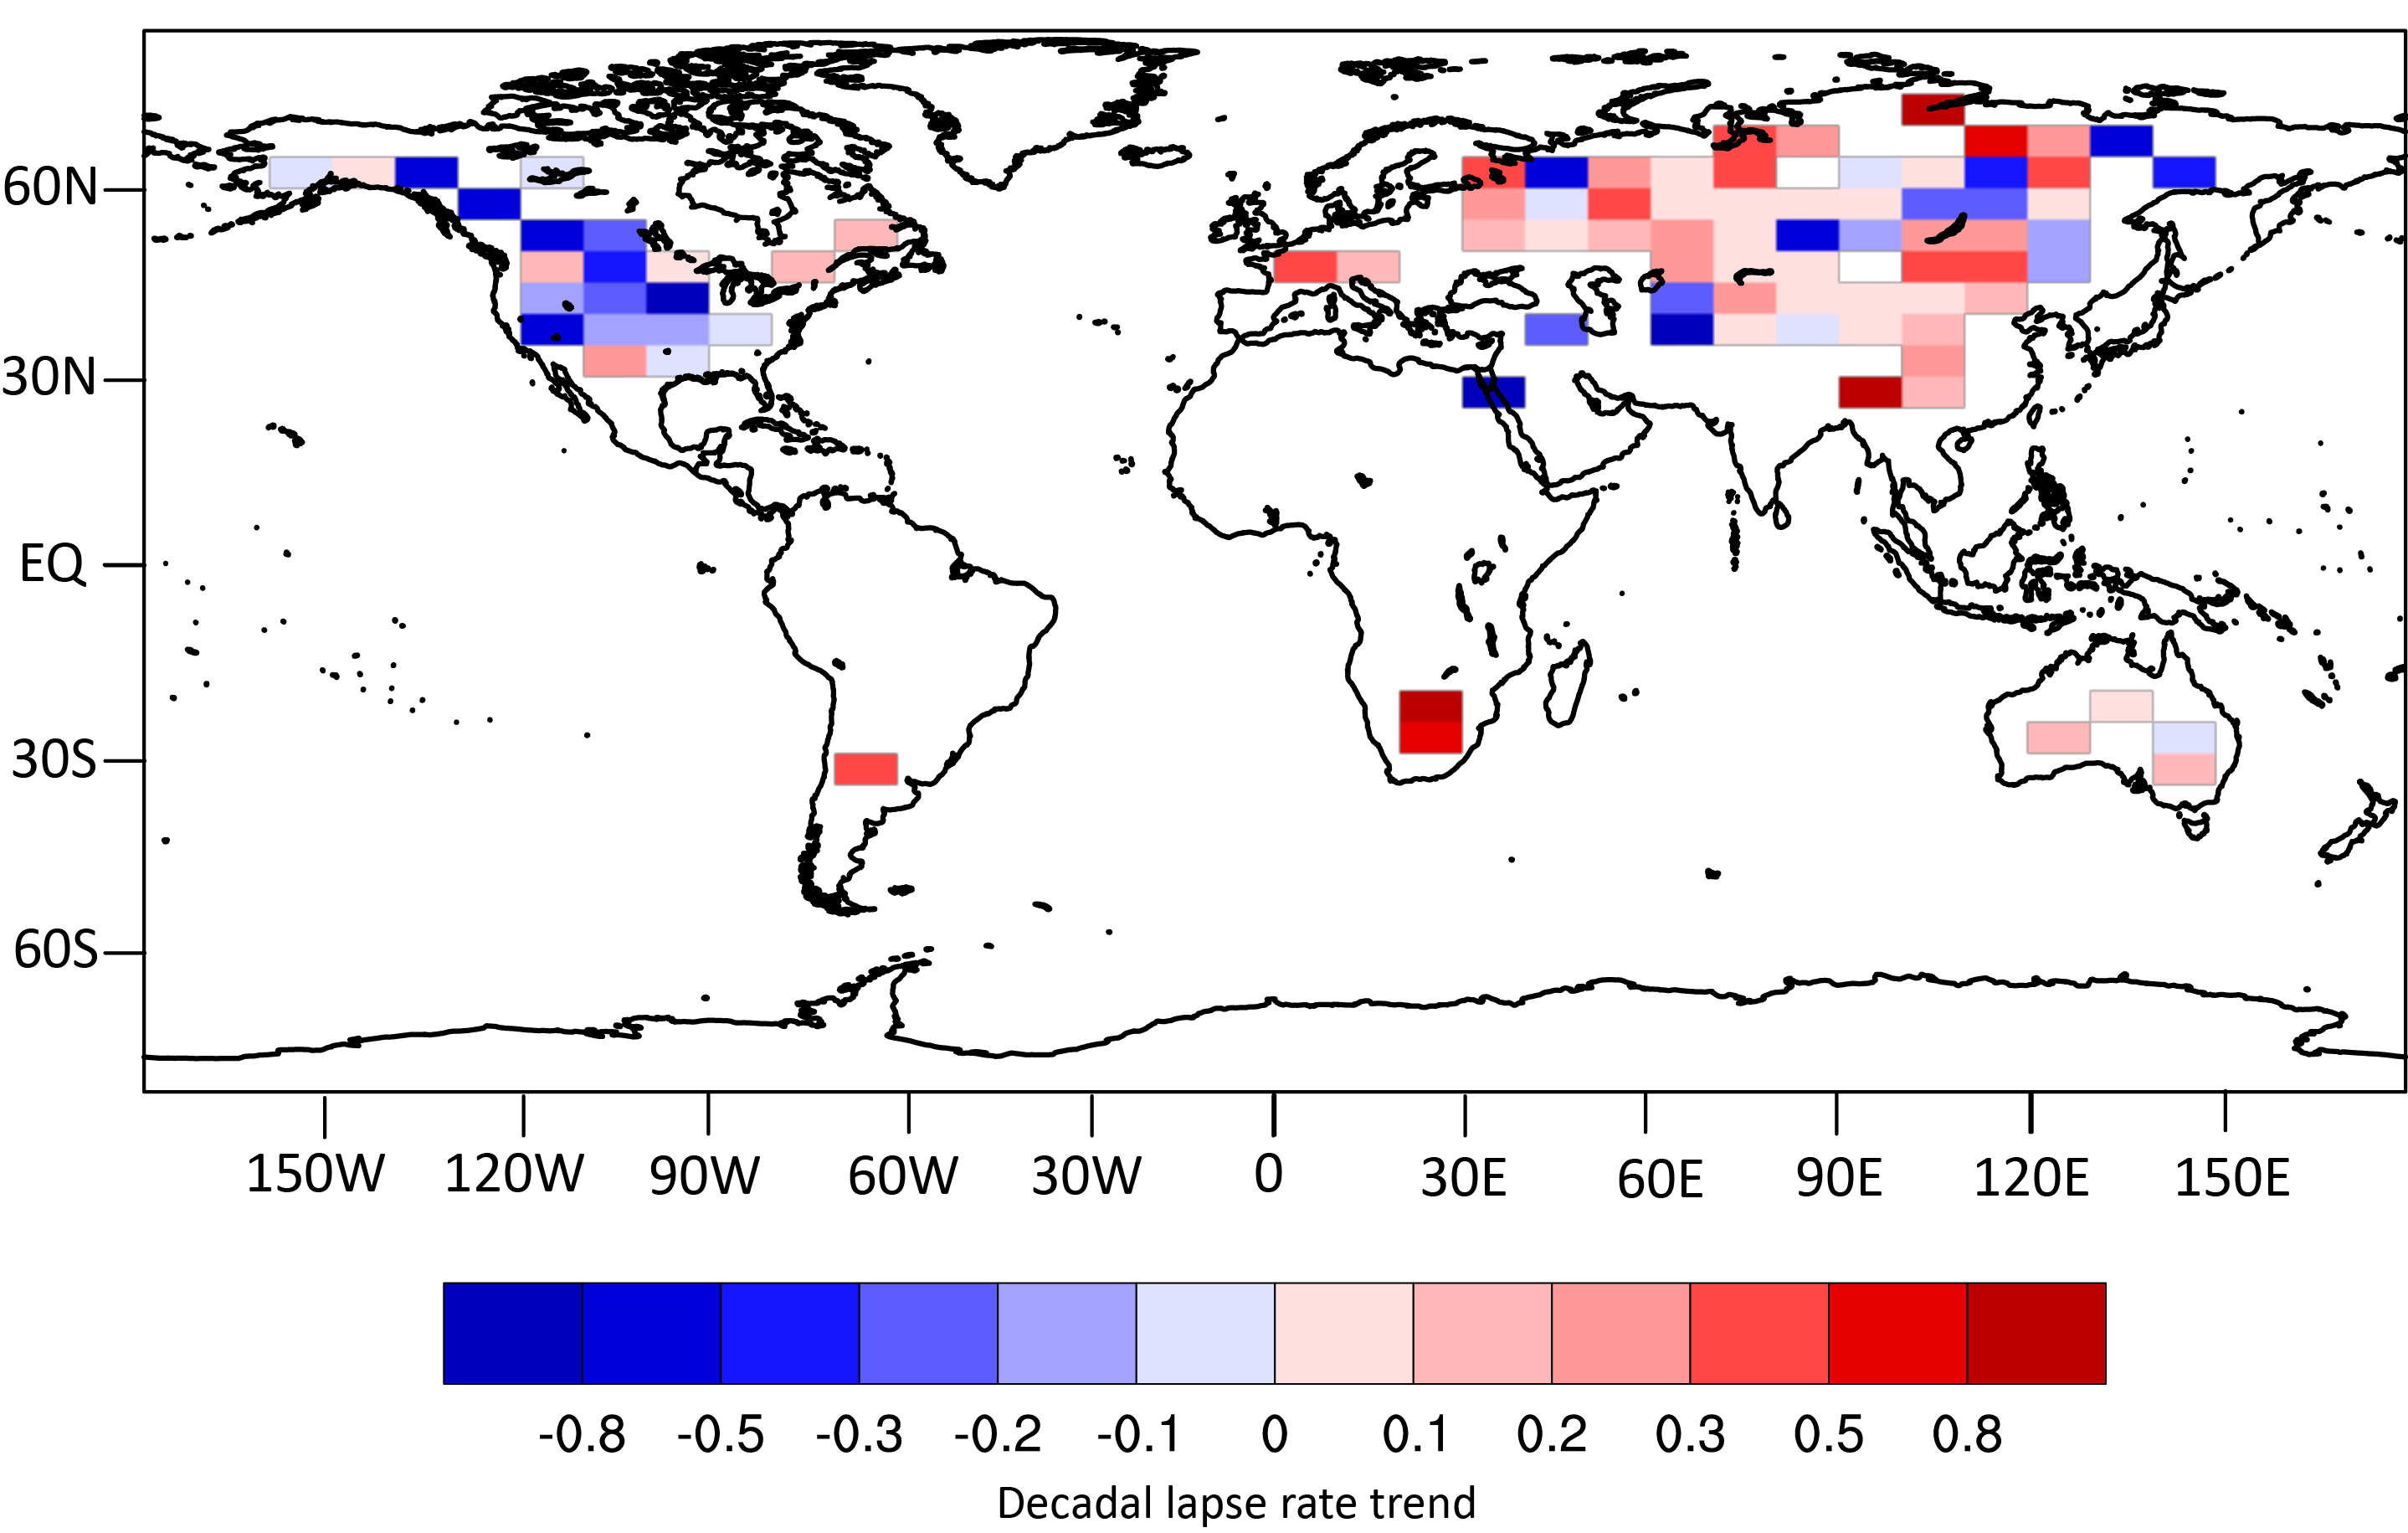
\includegraphics[width=1 \textwidth]{近地层温度垂直递减率趋势}
    \bicaption{近地层垂直温度递减率趋势( 每十年)}{Near surface lapse rate trend (in $decade^{-1})$}
        \label{fig:lapserate}
\end{figure}

\section{本章小结}

本章从城市化,植被变化和大气稳定度变化三个方面分析了大气运动阻力变化对于陆地地表风速长期变化的影响,得到以下结论:

\begin{enumerate}

\item 近30多年来全球特别是亚洲城市化进程迅猛,城市化速度与风速趋势呈显著负相关关系,表明城市化进程是地表风速减小的重要原因,模式试验结果表明珠江三角洲城市变化可以解释1979年来观测风速减小的35\%。

\item 近30多年来NDVI在北半球普遍呈增长趋势,表明植被普遍增加,但其与风速变化并没有很好的相关关系,原因可能是草地等低矮植被对10 m风速难以产生显著影响。在植被变化由林地变化主导的芬兰发现NDVI与风速趋势呈显著负相关,模式试验结果表明南芬兰林地变化可以解释1979年以来观测风速减小的87\%。

\item 北美日间垂直温度递减率普遍呈负趋势,预示着湍流活动减弱,高层动量难以向地表附近传递,这也解释了为何北美自由大气风速和地表风速趋势呈反向变化。欧洲和亚洲日间垂直温度递减率大部分呈现正趋势,预示湍流活动增强,高层动量更容易向地表附近传递。

\end{enumerate}